\documentclass[a4paper,10pt]{article}

%inputs
\usepackage[utf8]{inputenc}
\usepackage{hyperref}
\usepackage{graphicx}
\usepackage{listings}
\usepackage{amssymb}
\usepackage[colorinlistoftodos,prependcaption,textsize=tiny]{todonotes}
%\usepackage[]{natbib}
\usepackage{apacite}
\usepackage{csquotes}

\newcommand{\blankpage}{
\newpage
\thispagestyle{empty}
\mbox{}
\newpage
}

%opening
\title{Auslagerung der Ausführung von Methoden der HYPRE Bibliothek in ein Cloudsystem
Recherche und Literaturverzeichnis}
\author{Thomas Rückert}

\begin{document}

%settings
\newcommand{\mycheckbox}[0]{\makebox[0pt][l]{$\square$}\raisebox{0.15ex}{\hspace{0.1em}$\checkmark$}}
\newcommand{\myuncheckbox}[0]{\makebox[0em][l]{$\square$}\raisebox{0.15ex}{\hspace{0.1em}$ $}}

\newenvironment{boxed}[1]
{\begin{center}Definition\\
\begin{tabular}{|p{0.9\textwidth}|}
\hline\\
\textbf{#1}\\\\
}
{
\\\\\hline
\end{tabular} 
\end{center}
}

%title

\maketitle
\thispagestyle{empty}
\blankpage
\setcounter{page}{1}
\renewcommand{\thepage}{\roman{page}}

%abstract

\begin{abstract}
\todo{abstract formulieren}
\end{abstract}
\blankpage

%meta

\tableofcontents
\newpage

\listoffigures
\newpage

\listoftables
\newpage

\lstlistoflistings
\newpage

\listoftodos
\newpage

\setcounter{page}{1}
\renewcommand{\thepage}{\arabic{page}}

%content

\section{Einführung in die relevanten Themen}

\subsection{Allgemeines und Recherche zum Thema Cloud}

\todo{check das hier:}
\begin{itemize}
 \item nur innerhalb der cloud (ungeeignet): Light-weight remote communication for high-performance cloud networks \url{http://ieeexplore.ieee.org/document/6483669/}
 \item Performance Analysis of High Performance Computing Applications on the Amazon Web Services Cloud \url{http://ieeexplore.ieee.org/abstract/document/5708447/}
\end{itemize}

\subsubsection{Einführung und Grundbegriffe zu Cloudcomputing}

Entwicklung von monolitischen Systemen zu verteilten Anwendungen (SOA, Client/Server).
Ermöglicht Auslagerung kostenpflichtiger Berechnungen auf Server, `schwacher` Client kein Problem mehr.
Serverlast kann bei Anwendungen stark schwanken.
Zum Beispiel periodische Schwankungen Tag vs Nacht.
Klassischer Server muss die hohe Last stemmen, hat dann in anderen Perioden starken leerlauf.
Einmalige, sehr hohe Last bei besonderen Situationen (zum Beispiel durch einmalige, nicht wiederkehrende Sportevents wie Olympia/WM).
Klassischer Server könnte in diesem Zeitraum komplett ausfallen.
Cloud soll dynamische Resource sein, die sich je nach Bedarf skalieren kann.

\begin{figure}[htbp]
\centering
\caption{Übersicht Grundlagen Cloud Computing}
\label{fig:cloudComputingOverview}
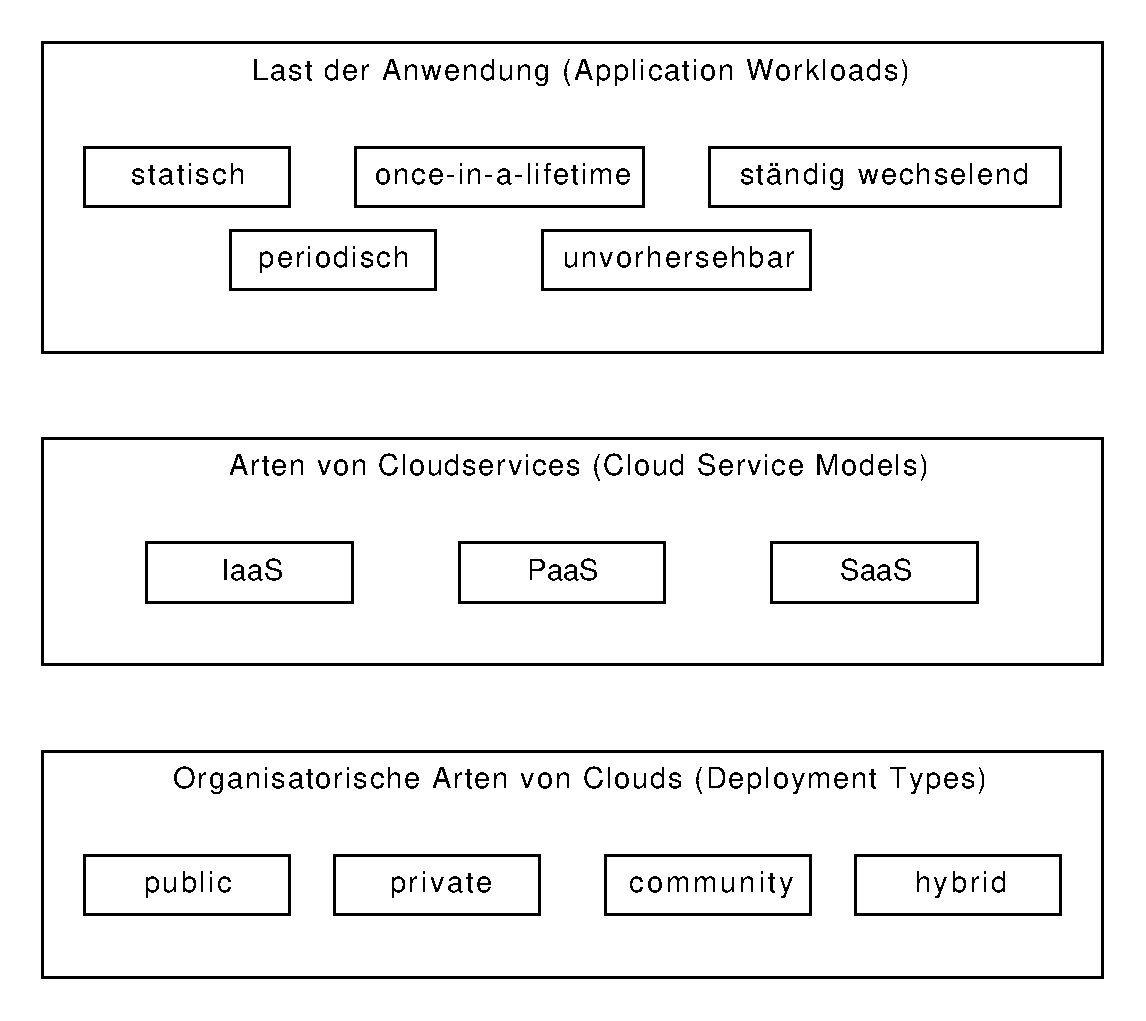
\includegraphics[width=\textwidth]{graphics/cloudComputingOverview.pdf}
\end{figure}

Im Folgenden werden die eben kurz angeschnittenen Eigenschaften von Cloudsystemen näher betrachtet.
Ein Übersicht dazu ist in Abbildung \ref{fig:cloudComputingOverview} gegeben.

\paragraph{Verteilung der Last von Anwendungen}

Im Buch Cloud Computing Patterns von Christoph Fehling wird die Verteilung von Last in die folgenden Kategorien eingeteilt:

\begin{itemize}
 \item static workload
 \item periodic workload
 \item once-in-a-lifetime workload
 \item unpredictable workload
 \item continuously changing workload
\end{itemize}

\textbf{Static workload} beschreibt eine nicht oder nur minimal schwankende Last.
\textbf{Periodic workload} hat dagegen wiederkehrende Schwankungen. Diese können zum Beispiel von der Tageszeit abhängig sein.
Ein \textbf{Once-in-a-lifetime workload} ist eine einmalige Lastspitze.
\textbf{Unpredictable workload} liegt vor, wenn sich die Last ständig, jedoch unregelmäßig und zufällig verändert, sodass diese nicht vorhersehbar ist.
\textbf{Continuously changing workload} verändert sich in linear steigend oder fallend.

\paragraph{NIST definition introduces five fundamental properties that characterize a cloud offering [CloudcomputingPatterns chap. 1.1]}

\begin{itemize}
 \item On-demand self-service
 \item Broad network access
 \item Measured service (pay-per-use)
 \item Resource pooling
 \item Rapid elasticity
\end{itemize}

\subparagraph{On-demand self-service}
`Provisioning` und `decomissioning` als Aktivitäten zum Hinzufügen oder Entfernen von weiteren Ressourcen.
Das kann durch Benutzer über grafische oder Kommandozeilenschnittstellen geschehen oder automatisiert über eine API.
\subparagraph{Broad network access}
Ein starkes Netzwerk \todo{genauer definieren} ist essentiell um eine Verbesserung durch die Auslagerung von Berechnungen zu erreichen. 
So kann Zugriffszeit auf Daten weniger abhängig von ihrem pysikalischen Speicherort werden.
\subparagraph{Measured service (pay-per-use)}
Durch die Nutzung von Cloudsystemen kann man stark von der Flexibilität der Ressourcen profitieren.
Diese Flexibilität muss sich auch im Bezahlmodell widerspiegeln.
\subparagraph{Resource pooling}
Ein Cloudsystem benötigt einen (großen \todo{genauer definieren}) Pool an Ressourcen.
Nur so kann Flexibilität für die Nutzer gewährleistet werden.
Um eine Austauschbarkeit der Ressourcen zu ermöglichen muss eine homogene Nutzung der Ressourcen existieren. \todo{warum? flexible Nutzung, Kosten}
\subparagraph{Rapid elasticity}
Elastizität von Cloudsystemen ermöglicht eine Effiziente Zuweisung von Ressourcen auf die Nutzer.
Der Ressourcepool muss dynamisch unter den Nutzern aufgeteilt werden können.

\paragraph{IDEAL cloud-native applications [CloudcomputingPatterns chap. 1.2]}

\begin{itemize}
 \item Isolated state
 \item Distribution
 \item Elasticity
 \item Automated management
 \item Loose coupling
\end{itemize}

\subparagraph{Isolated state}
Cloudanwendungen und ihre Komponenten sollten zustandslos sein.
Jede Ressource die zustandslos ist kann deutlich einfacher entfernt oder hinzugefügt werden als eine Ressource mit einem Zustand.
So können aufeinander folgende Interaktionen eines Nutzers beliebig auf verschiedene Ressourcen verteilt werden.
Eine Ressource die beispielsweise die erste Interaktion getätigt hat wird für weitere Interaktionen nicht mehr benötigt.
\subparagraph{Distribution}
Cloudsysteme können auf viele verschiedene Standorte verteilt sein.
In jedem Fall bestehen sie aus vielen verschiedenen Ressourcen.
Anwendungen sollten daher aus mehreren Komponenten bestehen, die auf verschiedene Ressourcen verteilt werden können.
\subparagraph{Elasticity}
Horizontale Skalierung statt vertikaler Skalierung:
Anwendung soll vom Hinzufügen weiterer Ressourcen profitieren können (horizontal).
Es soll nicht nur die `Verbesserung` einer Ressource eine bessere performance ermöglichen (vertikal).
Die Stärke von Cloudsystemen ist die dynamische Zuweisung von Ressourcen.
Cloudanwendungen müssen daher horizontal skalieren, also eine Parallelisierbarkeit vorweisen.
\subparagraph{Automated management}
Durch die Elastizität können Ressourcen von Cloudanwendungen während der Laufzeit ständig hinzugefügt und entfernt werden.
Diese Aktionen sollten aufgrund von Monitoring der Systemlast ausgelöst werden.
Damit die Verwaltung der Ressourcen jederzeit schnell und entsprechend der aktuellen Lage stattfindet sollte sie automatisiert sein.
\subparagraph{Loose coupling}
Da sich die verfügbaren Ressourcen der Anwendung während der Laufzeit ändern können sollten Komponenten möglichst unabhängig voneinander sein.
Das reduziert die Fehleranfälligkeit für die Fälle in denen Komponenten kurzzeitig nicht verfügbar sind. \todo{wie?}
Da verteilte Anwendung diese Eigenschaft aufweisen sind Technologien wie Webservices, SOA, asynchrone Kommunikation relevant für Cloudanwendungen. \todo{Technologien etwas weiter ausführen}

\subsubsection{Kategorisierung von Cloudsystemen}

\paragraph{Cloud Service Models}

\begin{itemize}
 \item Infrastructure as a Service (IaaS)
 \item Platform as a Service (PaaS)
 \item Software as a Service (SaaS)
\end{itemize}

\textbf{Infrastructure as a Service} gibt einem Zugang zu Netzwerk, Computern (unter umständen virtuell) und Speicher.
Es ist daher sehr nah an den schon länger existierenden und bekannten Hosted Server Lösungen. \todo{wie zum beispiel, kurz erläutern}
\textbf{Platform as a Service} dageben entfernt die Notwendigkeit die unterliegende Infrastruktur zu verwalten.
Das betrifft Hardware sowie die Betriebssystemebene.
Man erhält eine Umgebung in der man seine Anwendung ausführen kann, ohne sich um Themen wie Updates, Kapazitäten von Speicher und anderen Ressourcen oder ähnliche typische Adminaufgaben kümmern zu müssen.
\textbf{Software as a Service} stellt ein Cloudmodell dar, welches sich eher an Endnutzer richtet.
Man erhält Zugriff auf eine Komplette Anwendung, wie zum Beispiel einen Mailserver.
Bei dieser Variante muss sich der Nutzer um keinerlei Aufgaben der Verwaltung der Software kümmern.

\paragraph{Organisatorische Arten von Clouds (Deployment Types)}

\begin{itemize}
 \item public
 \item private
 \item community
 \item hybrid
\end{itemize}

Eine \textbf{public cloud} ist für jeden verfügbar.
Eine \textbf{private cloud} dagegen nur für ein einziges Unternehmen oder einen Nutzer (od. Interessengemeinschaft).
Eine \textbf{community cloud} liegt zwischen den beiden ersten Varianten. 
Sie ist in der Regel für eine Menge von Unternehmen verfügbar.
Das kann notwendig werden, falls die Unternehmen an einem gemeinsamen Projekt arbeiten.
Bei \textbf{hybrid clouds} ist von mehreren Clouds die Rede.
Diese können aus verschiedenen Arten bestehen und sind untereinander verbunden.
So können sich unterschiedliche Anwendungen unter eigenständigen Umgebungen Informationen austauschen und interagieren.

\subsubsection{Cloudsysteme}

\todo{Vergleich in Tabelle? - Konflikt zu chpt. 'Gegenüberstellungen ...'}

\paragraph{Verfügbare Cloudsysteme für public Clouds}

\subparagraph{Amazon EC2}

\url{https://www.youtube.com/watch?v=jLVPqoV4YjU&index=3&list=WL}
ssh Zugang siehe ab Minute 50

Instances mit verschiedenen verfügbaren Images = AMI (Linux, Windows).
ELB als elastischer Loadbalancer.
EBS - elastischer Blockstorage.
CloudWatch zum Überwachen von Ressourcen und Applikationen.
Kann zum automatischen Skalieren genutzt werden.
EC2 Actions - Recover, Stop, Terminate.
AWS CodeDeplay erlaubt deploying ohne downtime.
Amazon
Amazon EC2 Container Service ist ein Containermanagementservice zur Nutzung von Docker Containern.

Kostenloser Testzugang: \url{https://aws.amazon.com/free/}

\paragraph{Open Source Cloudsystem für private Clouds}

\begin{itemize}
 \item a guide to open source cloud \url{http://www.tomsitpro.com/articles/open-source-cloud-computing-software,2-754.html}
 \item 5 open source cloud platforms \url{http://solutionsreview.com/cloud-platforms/open-source-cloud-platforms-enterprise/}
\end{itemize}

\subparagraph{Sandstorm}

Link: \url{https://sandstorm.io/}\\

Kann als private oder public cloud genutzt werden.
Kann entweder im bestehenden Cloudsystem von Sandstorm genutzt werden oder selbst gehostet werden.
Im Cloudsystem von Sandstorm stehen SaaS und PaaS bereit.
Wenn man selbst hostet sind alle Service Modelle verfügbar, also zusätzlich auch IaaS.

Die verfügbaren Platformen stellen ein Linuxsystem bereit.
Daher kann jede beliebige Sprache genutzt werden welche auf Linux läuft.
Ist aber in erster Linie für SaaS-Apps gedacht.\\

Fazit:
wohl ungeeignet

\subparagraph{Openstack}

Link: \url{https://www.openstack.org/}\\
Openstack kostenlos testen: \url{http://trystack.org/}\\
devstack for getting started with openstack \url{http://docs.openstack.org/developer/devstack/}\\
install openstack on ubuntu \url{https://www.youtube.com/watch?v=jpk4i66-IU4}\\

why openstack? \url{https://www.youtube.com/watch?v=Bk4NoUsikVA}\\

Wird in erster Linie als IaaS verwendet.
Man kann bestehende Hardware mit Cloudstack in ein Cloudsystem umwandeln.
Es stehen verschiedene Services bereit, mit denen Kernanforderungen wie Speicher (Swift) oder Rechenleistung (Nova) befriedigt werden können.
Es gibt darüber hinaus weitere optionale Services für beispielsweise Datenbanken (Trove), Messaging (Zaqar), Container (Magnum) und viele Weitere.\\

Beispielkonfiguration: \url{https://www.openstack.org/software/sample-configs#high-throughput-computing}

GLANCE - Image Service
'Stores and retrieves virtual machine disk images. OpenStack Compute makes use of this during instance provisioning.'

NOVA - Compute
'Manages the lifecycle of compute instances in an OpenStack environment. Responsibilities include spawning, scheduling and decomissioning of machines on demand.'

KEYSTONE - Identity
'Provides an authentication and authorization service for other OpenStack services. Provides a catalog of endpoints for all OpenStack services.'

CINDER - Block Storage
'Provides persistent block storage to running instances. Its pluggable driver architecture facilitates the creation and management of block storage devices.'\\

Fazit:
modulare Services
passend für Anforderungen

\subparagraph{Apache Cloudstack}

\begin{boxed}{Apache Cloudstack \url{https://cloudstack.apache.org/}}
'Apache CloudStack is an open source Infrastructure-as-a-Service platform that manages and orchestrates pools of storage, network, and computer resources to build a public or private IaaS compute cloud.
\end{boxed}

\url{https://cloudstack.apache.org/}\\

With CloudStack you can:

Set up an on-demand elastic cloud computing service.
Allow end-users to provision resources' [http://docs.cloudstack.apache.org/en/latest/concepts.html]

private
IaaS

\subsubsection{Ressourcen}

\begin{itemize}
 \item amazon aws \url{https://aws.amazon.com/types-of-cloud-computing/}
 \item BOOK: cloud computing patterns \url{https://katalog.bibliothek.tu-chemnitz.de/Record/0012763915}
 \item raspberry pi private cloud \url{https://sc5.io/posts/a-private-raspberry-pi-cloud-with-arm-docker/}
 \item more raspberry \url{https://www.raspberrypi.org/forums/viewtopic.php?f=36&t=54997}
\end{itemize}

\subsection{Mathematische Grundlagen}

\paragraph{Laplace-Gleichung}
Partielle Differentialegleichung.
\todo{Grundlagen für HYPRE: 2D Laplace}
\url{https://www.youtube.com/watch?v=Z9NjA_f2VZw}
\url{https://www.youtube.com/watch?v=-D4GDdxJrpg}

\subsection{Parallele Programmierung}

Die absolute Ausführungszeit ist ein Hauptkriterium für die Performanz.
Sie sollte möglicht gering sein.
Ab einem gewissen Punkt kann die sequentielle Ausführung jedoch nicht mehr wesentlich optimiert werden.
Sollte es im Algorithmus jedoch unabhängige Berechnungen geben kann eine parallele Ausführung eine deutlich Verbesserung der Ausführungszeit erreichen.
Parallele Programme werden immernoch auf einem einzelnen Computer ausgeführt.
An der Ausführung sind mehrere Prozesse beteiligt.
Diese kommunizieren über einen gemeinsamen Speicher.

\paragraph{Grundbegriffe Paralleler Ausführung}

Die Ausführungszeit läuft bei einer parallelen Berechnung ab dem Start des Programmes bis die Ausführung des letzten teilnehmenden Prozessors beendet ist\cite{ppRauberRuenger}.
Diese Zeit nennt sich parallele Ausführungszeit $T_p(n)$, wobei $n$ die Problemgröße beschreibt.
Kriterien zur Bewertung eines parallelen Programmes sind Kosten, Speedup und Effizienz.

\subparagraph{Die Kosten}\cite[180]{ppRauberRuenger} $C_p(n)$ ergeben sich aus dem Produkt der parallelen Ausführungszeit $T_p(n)$ und der Anzahl der Prozessoren $p$:

\begin{center}
$C_p(n) = T_p(n) * p$
\end{center}

Die Kosten geben so die insgesamt notwendige Arbeit an.

\subparagraph{Der Speedup}\cite[180-182]{ppRauberRuenger} gibt die Verbesserung der parallelen Implementierung im Vergleich zur sequentiellen Implementierung an.
Er wird durch $S_p(n)$ beschrieben und ergibt sich aus der Division von der Ausführungszeit der besten sequentiellen Lösung $T^*(n)$ durch die parallele Ausführungszeit $T_p(n)$:

\begin{center}
$S_p(n) = \frac{T^*(n)}{T_p(n)}$
\end{center}

Der Speedup gibt somit die relative Ersparnis der parallelen Ausführung im Vergleich zur Sequentiellen an.

\subparagraph{Die Effizienz}\cite[182-183]{ppRauberRuenger} $E_p(n)$ ist ein Maß für die Performanz eines parallelen Programms.
Sie kann auf verschiedene Arten bestimmt werden:
Die Division besten sequentiellen Lösung $T^*(n)$ durch die Kosten $C_p(n)$.
Oder der Division des Speedup $S_p(n)$ durch die Anzahl der Prozessoren $p$.

\begin{center}
$E_p(n) = \frac{T^*(n)}{C_p(n)} = \frac{S_p(n)}{p}$
\end{center}

Eine optimale Effizienz wird durch den Wert 1 beschrieben $E_p(n) = 1$.
Diese wird erreicht wenn $S_p(n) = p$ ist.

\paragraph{Verteilte Ausführung}

Verteilte Systeme bestehen im Unterschied zur parallelen Programmierung.
Hierbei wird nicht mehr nur auf einem Computer gerechnet.
Es befinden sich stattdessen mehrere autonome in einem Netzwerk\cite{CS61A}.
Diese kommunizieren über den Austausch von Nachrichten.
Ein Standard für den Nachrichtenaustausch im verteilten sowie parallelen Rechnen ist das Message-Passing Interface - MPI\cite{MPIhome}.

\paragraph{MPI}


MPI wird beschrieben als \blockquote[{\cite[1]{mpi31report}}]{message-passing library interface specification}.


MPI definiert einen Standard für message passing Bibliotheken, also Nachrichtenübertragung.
Der Standard wird vom MPI Forum spezifiziert.
Er existiert in verschiedenen Versionen.
1994 wurde die erste Version veröffentlicht: MPI-1.0\cite[ii]{mpi31report}.
Die derzeit aktuellste Version ist MPI-3.1, welche seit 2015 existiert.



Es existiert eine Reihe von Implementierungen.
Drei frei verfügbare Beispiele sind MPICH, LAM/MPI und OpenMPI\footnote{MPICH: \url{http://www.mpich.org}, LAM/MPI: \url{http://www.lam-mpi.org}, OpenMPI: \url{http://www.open-mpi.org}}\cite[228]{ppRauberRuenger}.
Wobei LAM/MPI einer mehrerer Vorgänger von OpenMPI ist.



\todo{Nutzt MPI für Parallelisierbarkeit: MPI - Message Passing Interface.}

\subsection{HYPRE - Überblick über die Bibliothek}

HYPRE ist eine freie Software die vom Center for Applied Scientific Computing\cite{hypreCASC} entwickelt wird.
Dieses ist ein Teil der Organisation Lawrence Livermore National Laboratory\cite{hypreLLNL}, einer der wichtigsten staatlichen Forschungseinrichtungen der USA\cite{hypreDownload}.

HYPRE ist unter der GNU Lesser General Public License (Free Software Foundation) Version 2.1 lizensiert.
Diese ermöglicht die Benutzung der Bibliothek HYPRE sowohl in freier als auch proprietär lizensierter Software.
Der Funktionsumfang von HYPRE wird beschrieben als 'Scalable Linear Solvers and Multigrid Methods'.

Die aktuellste Version 2.11 ist seit dem 09.06.2016 verfügbar.
Die Bibliothek steht in dieser Version für die Sprachen C (nativ), C++ und FORTRAN bereit.
Bis zur vorletzten Minorversion 2.10 wurde HYRPE auch mit dem Babel Interface angeboten.
Dieses bot die Möglichkeit HYPRE von anderen Sprachen als C und FORTRAN zu nutzen.
So wurde im User Manual die Verwendung aus der Sprache Python beschrieben.
Seit Version 2.11.1 steht jedoch keine Implementierung mehr von HYPRE mit Babel Interface zur Verfügung.

\subsubsection{Funktionsumfang (und deren Funktionsweise)}

Wie bereits erwähnt wird der Funktionsumfang von HYPRE als 'Scalable Linear Solvers and Multigrid Methods' beschrieben.
Zur detaillierteren Erklärung von HYPRE kann man diese Beschreibung genauer Betrachten:

\paragraph{Begriffsklärung}

Der Begriff \textbf{Solver} beschreibt ein Stück Software, dieses kann beispielsweise als Bibliothek implementiert sein.
Mit Hilfe dieses Stücks Software kann man ein mathematisches Problem lösen.
Für ein Problem kann es verschiedene Implementierungen von \textbf{Solvern} geben.
Diese können bei unterschiedlichen Faktoren der Eingabedaten Vor- und Nachteile haben.
Diese können beispielsweise in Performance oder Genauigkeit liegen.

\textbf{Linear} beschreibt die Art von Problemen die HYPRE lösen kann.
Es handelt sich dabei um die lineare Algebra.
Ein wichtiger Teil der linearen Algebra sind lineare Gleichungssysteme.
\todo{erweitern}

Das zweite Adjektiv zum Begriff Solver ist \textbf{scalable}, also skalierbar.
Es gibt also einen Hinweis darauf, dass die Implementierungen der Solver in HYPRE auch oder besonders bei großen Eingaben eine gute Performanz aufweisen.
Für die Bewertung wird bei einer wachsenden Problemgröße ebenso die Rechenkapazität erhöht.
Skalierbarkeit einer Funktion liegt dann vor, wenn die nötige Ausführungszeit dabei konstant gehalten werden kann.\cite{Henson00boomeramg}
Dabei ist es in der Regel hilfreich, dass rechenintensive Teile parallel ausgeführt werden können.
Man spricht in diesem Fall von horizontaler Skalierung, also dem hinzufügen weiterer Berechnungsknoten.
Das können beispielsweise weitere Rechner sein die einem Cluster hinzugefügt werden.
Um dabei eine verbesserte Leistung zu erhalten muss die Software eine entsprechende Skalierung unterstützen.
Die Berechnungen müssen also in voneinander unabhängige Teile gespalten werden können.
Im Gegensatz dazu steht die vertikale Skalierung.
Hier hat man eine einzige Ressource deren Rechenleistung erhöht wird.
Diese ist für eine Software in der Regel einfacher zu nutzen, stößt allerdings schneller an Grenzen.
So kann die die Signalfrequenz einer CPU zum Beispiel nicht beliebig weit erhöht werden.

Der zweite Teil der Beschreibung lautet \textbf{Multigrid Methods} steht für Mehrgitterverfahren.
Diese stellen eine Approximationslösung für Differentialgleichungen dar.
Dafür werden die Eingabedaten auf eine Weise ausgedünnt, bei der sich die Lösung so wenig wie möglich verändert.
Eine solche Verkleinerung der Daten ist bei Problemen mit bis zu Milliarden von Unbekannten wichtig.
So kann die Komplexität von Problemen erheblich reduziert werden.
HYPRE verwendet beispielsweise Algebraic Multigrid Methods (AMG).

Eine parallele Implementierung davon ist \textbf{BoomerAMG}.
Dieser wurde bereits für Probleme mit dutzenden Millionen Unbekannten auf Maschinen mit über Tausend Prozessoren eingesetzt.\cite{Henson00boomeramg}
Mehrgitterverfahren können als sogenannte Preconditioner, oder Vorkonditionierer, eingesetzt werden.
Dabei werden die Eingabedaten noch vor dem Lösen optimiert.
BoomerAMG kann beispielsweise direkt als Solver verwendet werden.
Ebenso kann es aber auch als Preconditioner verwendet werden und anschließend ein anderer Solver zum Einsatz kommen.
Beispielsweise bei der Verwendung des Krylow-Unterraum-Verfahren ist eine Vorkonditionierung wichtig. 
Dieses ist auf das Lösen dünnbesetzter Gleichungssysteme optimiert.
Wenn die Eingabedaten diesem Kriterium nicht entsprechen sollten sie also zunächst mit einem anderen Verfahren vorkonditioniert werden.

Im wesentlichen stellt HYPRE also Funktionen zum Lösen linearer Algebra bereit.
Diese sind soweit optimiert, dass sie skalieren.
Die Performanz der Berechnungen kann durch Mehrgitterverfahren verbessert werden.
BoomerAMG ist ein Beispiel für ein solches Verfahren welches parallelisierbar ist.

\paragraph{Performanz}
Nutzt MPI für Parallelisierbarkeit: MPI - Message Passing Interface.

\todo{performance}

\paragraph{Conceptual Interfaces}
\paragraph{Solver Strategies}
\paragraph{Preconditioner(s)}

Preconditioning	\cite{FritzschePreconditioning}

\subsubsection{Verwendung und Implementierung}

\paragraph{Installation}
Um HYPRE zu installieren sind einige Abhängigkeiten zu erfüllen.
Die nötigen Schritte in einem Ubuntu sehen wie folgt aus:
\begin{lstlisting}[frame=single,caption=Installation HYPRE in Ubuntu]
cd /vagrant

//yaourt mpich2
//yaourt openmpi
sudo apt-get install mpich

//Download https://github.com/LLNL/hypre
git clone https://github.com/LLNL/hypre

//Innerhalb des Verzeichnis muss `configure` 
//gefolgt von einem `make` ausgeführt werden. 
cd hypre/src

./configure

//Alternativ kann auch das build tool CMake 
//eingesetzt werden.
make
\end{lstlisting}

\paragraph{Implementierung}

\paragraph{Checkliste}

Die folgenden Punkte beschreiben grob die notwendigen Schritte eines Workflows für die Implementierung.

\begin{enumerate}
 \item Build any necessary auxiliary structures for your chosen conceptual interface. /
 Datenstrukturen für Gitter (Grid) und Schablone (Stencil) aufbauen, abhängig vom gewählten Interface.
 \item Build the matrix, solution vector, and right-hand-side vector through your chosen conceptual interface. /
 Matrix, Lösungsvektor, right-hand-side Vektor aufbauen. 
 Diese können über verschiedene HYPRE-calls mit den jeweiligen Informationen gefüllt werden.
 \item Build solvers and preconditioners and set solver parameters (optional). /
 Solver und preconditioner aufbauen und deren Parameter setzen.
 Je nach conceptual interface sind verschiedene solver verfügbar.
 \item Call the solve function for the solver. /
 Solver aufrufen damit das Problem berechnet wird.
 \item Retrieve desired information from solver. /
 Lösung vom solver abrufen.
\end{enumerate}

Zunächst müssen die Datenstrukturen für die In- und Outputdaten definiert werden.
Dies können beispielsweise Matrizen oder Vektoren sein.
Die Entscheidung über das Inputformat ist abhängig vom gewählten Input-Interface.

Die gewählten Datenstrukturen müssen als nächstes mit den Inputdaten gefüllt werden.
HYPRE stellt dafür verschiedene Calls bereit.
\todo{beispiele}

Der nächste Schritt ist das Anlegen des gewünschten Solvers.
Es stehen verschiedene Solver bereit\cite{hypreManual}, beispielsweise SMG (a parallel semicoarsening multigrid solver) oder BoomerAMG (parallel implementation of the algebraic multigrid method).

\subsubsection{Beispielhafter Einblick}

In der HYPRE-Bibliothek steht eine Reihe von Beipielen für die Benutzung zur Verfügung.
An dieser Stelle wird das Beispiel 5 näher betrachtet.
Dieses löst ein zweidimensionales Laplaceproblem (nxn) ohne Randbedingungen.
Die Anzahl der Unbekannten beträgt daher N=n².
Die komplette Implementierung des Beispiel 5 ist im Anhang zu finden.

\paragraph{Vorbereitungen}

Da HYPRE für die Parallelisierung auf die MPI Bibliothek zurückgreift muss dieses auch zu Beginn der Anwendung initialsiert werden.
Dafür muss durch \begin{verbatim}MPI_INIT()\end{verbatim} eine grundsätzliche MPI-Session gestartet werden.
Weiterhin müssen für die Prozesse ein Kommunikator bestimmt und die eigene id sowie die gesamte Anzahl der Prozesse gelesen werden.
Dafür werden die Methoden \begin{verbatim}MPI_Comm_rank()\end{verbatim} und \begin{verbatim}MPI_Comm_size()\end{verbatim} aufgerufen.

\begin{lstlisting}[frame=single,caption=HYPRE Nutzung: Vorbereitungen]

//init mpi
MPI_Init(&argc, &argv);
MPI_Comm_rank(MPI_COMM_WORLD, &myid);
MPI_Comm_size(MPI_COMM_WORLD, &num_procs);

\end{lstlisting}

\paragraph{Matrix anlegen (analog zu Vektor)}

Matrizen und Vektoren anlegen.
Es stehen analoge Methoden für Matrizen und Vektoren bereit.
Im folgenden Listing \ref{HYPRENutzungMatrix} sind die wichtigen Methoden daher lediglich für das Beispiel der Matrix aufgeführt.

\begin{lstlisting}[frame=single,caption=HYPRE Nutzung: Matrix anlegen (analog dazu Vektor), label=HYPRENutzungMatrix]
//create matrix / vector

HYPRE_IJMatrix A;
int ilower;
int iupper;

//...

/* Create the matrix.
  Note that this is a square matrix, so we indicate the row partition
  size twice (since number of rows = number of cols) */
HYPRE_IJMatrixCreate(MPI_COMM_WORLD, ilower, iupper, ilower, iupper, &A);

/* Choose a parallel csr format storage (see the User's Manual) */
HYPRE_IJMatrixSetObjectType(A, HYPRE_PARCSR);

/* Initialize before setting coefficients */
HYPRE_IJMatrixInitialize(A);

//in einem loop:
HYPRE_IJMatrixSetValues(A, 1, &nnz, &i, cols, values);

/* Assemble after setting the coefficients */
HYPRE_IJMatrixAssemble(A);

/* Get the parcsr matrix object to use */
HYPRE_IJMatrixGetObject(A, (void**) &parcsr_A);

\end{lstlisting}

\paragraph{Solver anlegen und aufrufen}

Solver erstellen und aufrufen.

\begin{lstlisting}[frame=single,caption=HYPRE Nutzung: Solver anlegen und aufrufen]
//create solver
//(Boomer)

/* Create solver */
HYPRE_BoomerAMGCreate(&solver);

/* Now setup and solve! */
HYPRE_BoomerAMGSetup(solver, parcsr_A, par_b, par_x);
HYPRE_BoomerAMGSolve(solver, parcsr_A, par_b, par_x);

/* Destroy solver object */
HYPRE_BoomerAMGDestroy(solver);

\end{lstlisting}

\paragraph{mit Preconditioner}

Solver mit anderem Preconditioner.

\begin{lstlisting}[frame=single,caption=HYPRE Nutzung: Solver mit Preconditioner]
//erstelle PCG mit AMG als preconditioner

/* Create solver */
HYPRE_ParCSRPCGCreate(MPI_COMM_WORLD, &solver);

/* Now set up the AMG preconditioner and specify any parameters */
HYPRE_BoomerAMGCreate(&precond);

/* Set the PCG preconditioner */
HYPRE_PCGSetPrecond(solver, (HYPRE_PtrToSolverFcn) HYPRE_BoomerAMGSolve,
                          (HYPRE_PtrToSolverFcn) HYPRE_BoomerAMGSetup, precond);

/* Now setup and solve! */
HYPRE_ParCSRPCGSetup(solver, parcsr_A, par_b, par_x);
HYPRE_ParCSRPCGSolve(solver, parcsr_A, par_b, par_x);

/* Destroy solver and preconditioner */
HYPRE_ParCSRPCGDestroy(solver);
HYPRE_BoomerAMGDestroy(precond);

\end{lstlisting}

\paragraph{weitere Parameter}

Vor dem Ausführen des solvers können weitere Parameter gesetzt werden.

\begin{lstlisting}[frame=single,caption=HYPRE Nutzung: Solver mit Preconditioner]
/* Set some parameters (See Reference Manual for more parameters) */
HYPRE_BoomerAMGSetPrintLevel(solver, 3);  /* print solve info + parameters */
HYPRE_BoomerAMGSetOldDefault(solver); /* Falgout coarsening with modified classical interpolaiton */
HYPRE_BoomerAMGSetRelaxType(solver, 3);   /* G-S/Jacobi hybrid relaxation */
HYPRE_BoomerAMGSetRelaxOrder(solver, 1);   /* uses C/F relaxation */
HYPRE_BoomerAMGSetNumSweeps(solver, 1);   /* Sweeeps on each level */
HYPRE_BoomerAMGSetMaxLevels(solver, 20);  /* maximum number of levels */
HYPRE_BoomerAMGSetTol(solver, 1e-7);      /* conv. tolerance */
\end{lstlisting}

\paragraph{Ergebnis auswerten}

Nach dem Lösen des Problems können die Ergebnisse gelesen werden.

\begin{lstlisting}[frame=single,caption=HYPRE Nutzung: Solver mit Preconditioner]
/* Run info - needed logging turned on */
HYPRE_BoomerAMGGetNumIterations(solver, &num_iterations);
HYPRE_BoomerAMGGetFinalRelativeResidualNorm(solver, &final_res_norm);
\end{lstlisting}

\paragraph{Alles zusammenfügen}

Im Anhang ist das komplette Beispiel 5 zu sehen, welches zuvor in Ausschnitten erläutert wurde.
Im folgenden soll der Zusammenhang der einzelnen Methoden näher erläutert werden.
\todo{näher erläutern, paragraphen oben drüber: methoden etwas genauer erklären}
\cite{hypreReferenceManual}

\subsubsection{Ressourcen}

\begin{itemize}
 \item offiziell: \url{http://computation.llnl.gov/projects/hypre-scalable-linear-solvers-multigrid-methods}
 \item Übersicht Publikationen: \url{http://computation.llnl.gov/projects/hypre-scalable-linear-solvers-multigrid-methods/publications}
 \item Pursuing scalability for hypre's conceptual interfaces \url{http://dl.acm.org/citation.cfm?doid=1089014.1089018}
 \item (mehr) beispiele \url{https://redmine.scorec.rpi.edu/anonsvn/fastmath/docs/ATPESC_2013/Exercises/hypre/examples/README_files/c.html}
\end{itemize}

\subsection{Webtechnologien und Werkzeuge für die verteilte Ausführung}

\subsubsection{RPC}

RPC steht für Remote Procedure Call.
In klassischen Programmen werden Funktionsaufrufe (oder Prozeduraufrufe) auf einem einzelnen Gerät mit einem einzigen Prozess durchgeführt.
Ein Schritt zur parallelen Ausführung ist die Interprozesskommunikation, bei der verschiedene Prozesse eines Systems miteinander kommunizieren können.
RPC geht noch einen Schritt weiter.
Die kommunizierenden Prozesse befinden sich hier in verschiedenen Adressräumen, können sich also auf verschiedenen Geräten befinden.
Der besondere Gedanke hinter RPC ist der, dass diese Aufrufe entfernter Programme Funktions- oder Prozedurbezogen erfolgen sollen.
Anstatt also eine Funktion aufzurufen und lokal auszuführen, soll sie auf einem entfernten System ausgeführt werden.
Die Implementierung mit RPC soll sich nicht weiter vom Programmablauf mit lokalen Funktionen unterscheiden.
Dennoch sind einige Unterschiede notwenig, um die Verbindung aufzubauen und zu verwalten.
Es unterscheidet sich hier von anderen Kommunikationsprotokollen wie REST\todo{was ist rest}, welches eine ressourcenbezogene Kommunikation verwendet.

\subsubsection{Service/Webservice}
\todo{erklärung service kommunikation allgemein}
SOAP

\subsubsection{Socket}
\todo{erklärung socket allgemein}

\newpage













\section{Implementierungen von Webtechnologien}

\subsection{RPC}

\todo{rpc aufräumen}

RPC steht für Remote Procedure Call.
Sie bieten die Möglichkeit von Funktionsaufrufen in verteilten Systemen.
Im Gegensatz zu Protokollen wie REST sieht RPC wie ein Methodenaufruf aus.
Das Ziel ist die Ausführung einer bestimmten Prozedur, nicht das verwalten einer bestimmten Ressource.
Protokolle sind zum Beispiel XML-RPC und Json-RPC.

\begin{itemize}
 \item understanding rest and rpc for http \url{https://www.smashingmagazine.com/2016/09/understanding-rest-and-rpc-for-http-apis/}
 \item Implementing remote procedure calls \url{http://dl.acm.org/citation.cfm?id=357392}
 \item c++ json-rpc lib \url{https://github.com/cinemast/libjson-rpc-cpp/}
\end{itemize}

\paragraph{REST vs RPC}

\todo{skizze rpc call (vs skizze rest call)}
\todo{warum rest ungeeignet}

\paragraph{XML-RPC}

XML-RPC ist ein Protokoll für Remote Procedure Calls.
In diesem wird XML zur Formatierung der übertragenen Daten verwendet.
Wie in RPC besteht auch in XML-RPC der Bezug auf Methoden.
Darin besteht der Unterschied zu anderen Protokollen, welche sich auf die Manipulation von Daten beziehungsweise Ressourcen beziehen.
Es gibt in verschiedenen Sprachen Implementierungen von Server-Client-Frameworks die das XML-RPC Protokoll zur Kommunikation verwenden.

\subparagraph{xml-rpc}

XML-RPC Bibliothek für C und C++ \url{http://xmlrpc-c.sourceforge.net/}.

Installation: \\
\begin{lstlisting}[frame=single,caption=XML-RPC Installation]
./configure
make
make install
//And then, if Linux:
ldconfig
\end{lstlisting}

Diese Bibliothek bietet ein performantes Framework zur Implementierung von XML-RPC Anwendungen.
Sie bietet sicher Kommunikation per HTTPS.
Es können größere Datenmengen per Packet Stream übertragen werden.
Die Verwendung der Frameworkmethoden erfolgt sehr transparent und modular, wodurch man leicht Einfluss auf die funktionsweise nehmen kann.
Das führt allerdings auch dazu, dass im Vergleich zu modernen Frameworks recht viel boiler plate code erforderlich ist.

\paragraph{JSON-RPC}

JSON-RPC ist wie XML-RPC ein Protokoll für Remote Procedure Calls.
Dieses verwendet für die Formatierung der Daten das Json-Format, was den wesentlichen Unterschied zum XML-RPC darstellt.
Das Json-Format benötigt im Vergleich zu XML wesentlich weniger Zeichen für die Strukturierung der Daten.
Durch die unterschiedliche Effizienz in der Repräsentation der Daten ergeben sich bei JSON-RPC bessere Übertragungsgeschwindigkeiten.
Die Auswahl an JSON Bibliotheken welche in C und C++ implementiert sind ist groß.
Im folgenden github-Projekt wurde eine große Auswahl miteinander verglichen: \url{https://github.com/miloyip/nativejson-benchmark}.

\todo{liste durchgehen}
\begin{itemize}
 \item information: \url{http://www.simple-is-better.org/json-rpc/}
 \item wiki: \url{https://en.wikipedia.org/wiki/JSON-RPC}
 \item json rpc server: \url{https://github.com/hmng/jsonrpc-c}
 \item tcp client: \url{http://jsonrpc-cpp.sourceforge.net/index.php?n=Main.HomePage}
 \item rpc client?: \url{https://groups.google.com/forum/#!topic/json-rpc/9O1dbQehU04}
\end{itemize}

Im folgenden Abschnitt wird eine Auswahl von JSON-RPC Bibliotheken vorgestellt:

\subparagraph{json-rpc}

json-rpc-libs:
\begin{itemize}
 \item \url{https://github.com/yeryomin/libjrpc}
 \item \url{https://github.com/jhlee4bb/jsonrpC}
 \item \url{https://github.com/hmng/jsonrpc-c}
 \item \url{https://github.com/pijyoi/jsonrpc}
\end{itemize}

\subparagraph{yeryomin/libjrpc}

\url{https://github.com/yeryomin/libjrpc}

install:

\begin{lstlisting}[frame=single,caption=yeryomin/libjrpc Installation]
git clone git@github.com:yeryomin/libjrpc.git
git clone git@github.com:yeryomin/libipsc.git
git clone git@github.com:yeryomin/libfmt.git
git clone git@github.com:zserge/jsmn.git
git clone git@github.com:yeryomin/liba.git

cd libipsc
make
sudo ln -s /path/to/libipsc.h /usr/include
cd ..

cd jsmn
make
sudo ln -s /path/to/jsmn.h /usr/include
cd ..

cd libfmt
make
sudo ln -s /path/to/libfmt.h /usr/include
cd ..

cd libjrpc
make
sudo ln -s /path/to/libjrpc.h /usr/include
\end{lstlisting}

so many unresolved dependencies.............. wow

\subparagraph{jhlee4bb/jsonrpC}

(needs libwebsockets installed: `yaourt libwebsockets` etc.)

\begin{lstlisting}[frame=single,caption=jhlee4bb/jsonrpC Installation]
git clone git@github.com:jhlee4bb/jsonrpC.git
cd jsonrpC
mkdir build
cd build
cmake ..
make
build output left in jsonrpc-x.y
\end{lstlisting}

völlig veraltet - websocket-lib ist inziwschen komplett inkompatibel

\todo{client and server stubs: \url{https://github.com/masroorhasan/RPC}}
\todo{rpc for php and c: \url{https://github.com/laruence/yar}}

\subsection{Bibliotheken/Frameworks/Implementierungen}

\subparagraph{Mercury}

Homepage: \url{https://mercury-hpc.github.io/}
Dokumentation: \url{http://mercury-hpc.github.io/documentation/}
High-level RPC Layer: \url{http://mercury-hpc.github.io/documentation/#high-level-rpc-layer}
Mailing-List: \url{https://lists.mcs.anl.gov/mailman/private/mercury/}

Für HPC optimierte c-Bibliothek.
Bietet außerdem MPI-Unterstützung.
(Etwas) Dokumentation vorhanden.

\subparagraph{Trios/Nessie}

\url{https://software.sandia.gov/trac/nessie/wiki/WikiStart}

\subparagraph{Portals}

\url{https://www.researchgate.net/publication/221201996_Efficient_Data-Movement_for_Lightweight_IO}

\subparagraph{DART}

\url{http://coewww.rutgers.edu/www4/cacweb/TASSL/Papers/dart_hpdc.pdf}
% \url{https://www.researchgate.net/publication/220717741_DART_a_substrate_for_high_speed_asynchronous_data_IO}

\subsection{andere}

\paragraph{Python in C Ausführen}

\subparagraph{ressourcen}

\url{https://docs.python.org/2.5/ext/callingPython.html}
\url{https://www.codeproject.com/articles/11805/embedding-python-in-c-c-part-i}

better

\url{http://www.linuxjournal.com/article/8497}
\url{https://www.codeproject.com/articles/820116/embedding-python-program-in-a-c-cplusplus-code}

\subparagraph{basics}

some text

\begin{lstlisting}[frame=single,caption=Python in C ausführen]
#include <python3.6m/Python.h>

int main()
{
  Py_Initialize();
  PyRun_SimpleString(
    "print('Hello World from Embedded Python.')"
  );
  Py_Finalize();
}
\end{lstlisting}

kompilieren von c-code mit python3.6

\begin{lstlisting}[frame=single,caption=Python in C kompilieren]
cc prog.c -o prog.o -I/usr/include/python3.6m -lpython3.6m 
  -lm -L/usr/lib/python3.6
\end{lstlisting}

\paragraph{spring-server framework}

\url{https://github.com/bartobri/spring-server}

\begin{lstlisting}[frame=single,caption=Installation bartobri/spring-server]
git clone git@github.com:bartobri/spring-server.git
\end{lstlisting}

\subsection{Serialisierung}

\url{https://www.quora.com/Is-there-a-C-struct-to-JSON-generator-library}

\paragraph{Protocol Buffers}

\todo{protobuf überarbeiten und nach oben zu grpc verweisen}

protobuf: \url{https://github.com/protobuf-c/protobuf-c-rpc}

\url{https://developers.google.com/protocol-buffers/}
Protocol buffers are a language-neutral, platform-neutral extensible mechanism for serializing structured data.
Implementierung für C:
\url{https://github.com/protobuf-c/protobuf-c}
\url{https://github.com/protobuf-c/protobuf-c-rpc}

\subparagraph{Fazit}

Generiert den Code für structs selbstständig.
Für den Anwendungsfall bestehen die Strukturen jedoch bereits und müssen umgewandelt werden.
Ist daher ungeeignet.

\subsection{Beispielinstallation OpenStack: Devstack}

\todo{Nova, Horizon ...}

Devstack ist ein Projekt von OpenStack, welches eine Grundinstallation einer OpenStack-Umgebung bereitstellen soll.
Es soll helfen eine Entwicklungsumgebung für OpenStack mit wenigen Schritten einzurichten.
DevStack ist nicht für den Produktiveinsatz vorgesehen.

In der Grundstruktur verschiedener Cloudsysteme gibt es starke Überschneidungen. 
Es gibt eine Menge von Hardwareressourcen die zur Verfügung stehen.
Dazu zählen Beispielsweise CPUs, RAM oder Speicher.
Es gibt weiterhin Instanzen von virtuellen Containern.
Diese Container beinhalten alles notwendige, um Software ausführen zu können.
Sie sind sehr leichtgewichtig und schlank.
\todo{evtl docker container ausführlicher}
Das liegt daran, dass sie kein komplettes eigenes Betriebssystem mitbringen.
Dies stellt den Hauptunterschied zu herkömmlichen Virtuellen Maschinen dar.

\url{http://docs.openstack.org/developer/devstack/}\\
\url{https://www.youtube.com/watch?v=jpk4i66-IU4}\\
\url{http://ronaldbradford.com/blog/setting-up-ubuntu-on-virtualbox-for-devstack-2016-03-30/}\\
\url{http://ronaldbradford.com/blog/setting-up-ubuntu-using-vagrant-2016-04-01/}\\
\url{http://ronaldbradford.com/blog/downloading-and-installing-devstack-2016-04-02/}\\

Automatisches Setup: \url{https://github.com/lorin/devstack-vm}

\paragraph{Grafische Oberfläche}

Die Oberfläche besteht aus drei großen Bereichen: Project, Admin und Identity.
Diese können am linken Rand ausgewählt werden.
Wichtig ist der Project-Bereich, in dem die Projekteigenschaften abgerufen und geändert werden können.

\subparagraph{Overview}

Eine gute Übersicht über den aktuellen Zustand des Projekts bietet hier die Seite 'Overview'.
In Abbildung \ref{fig:devstack:overview} ist ein Screenshot zu sehen.
Diese zeigt einen Überblick über Instances, VCPUs, RAM, Floating IPs, Security Groups, Volumes und Volume Storage.

\begin{figure}[htbp]
\centering
\caption{Überblick über die Cloud}
\label{fig:devstack:overview}
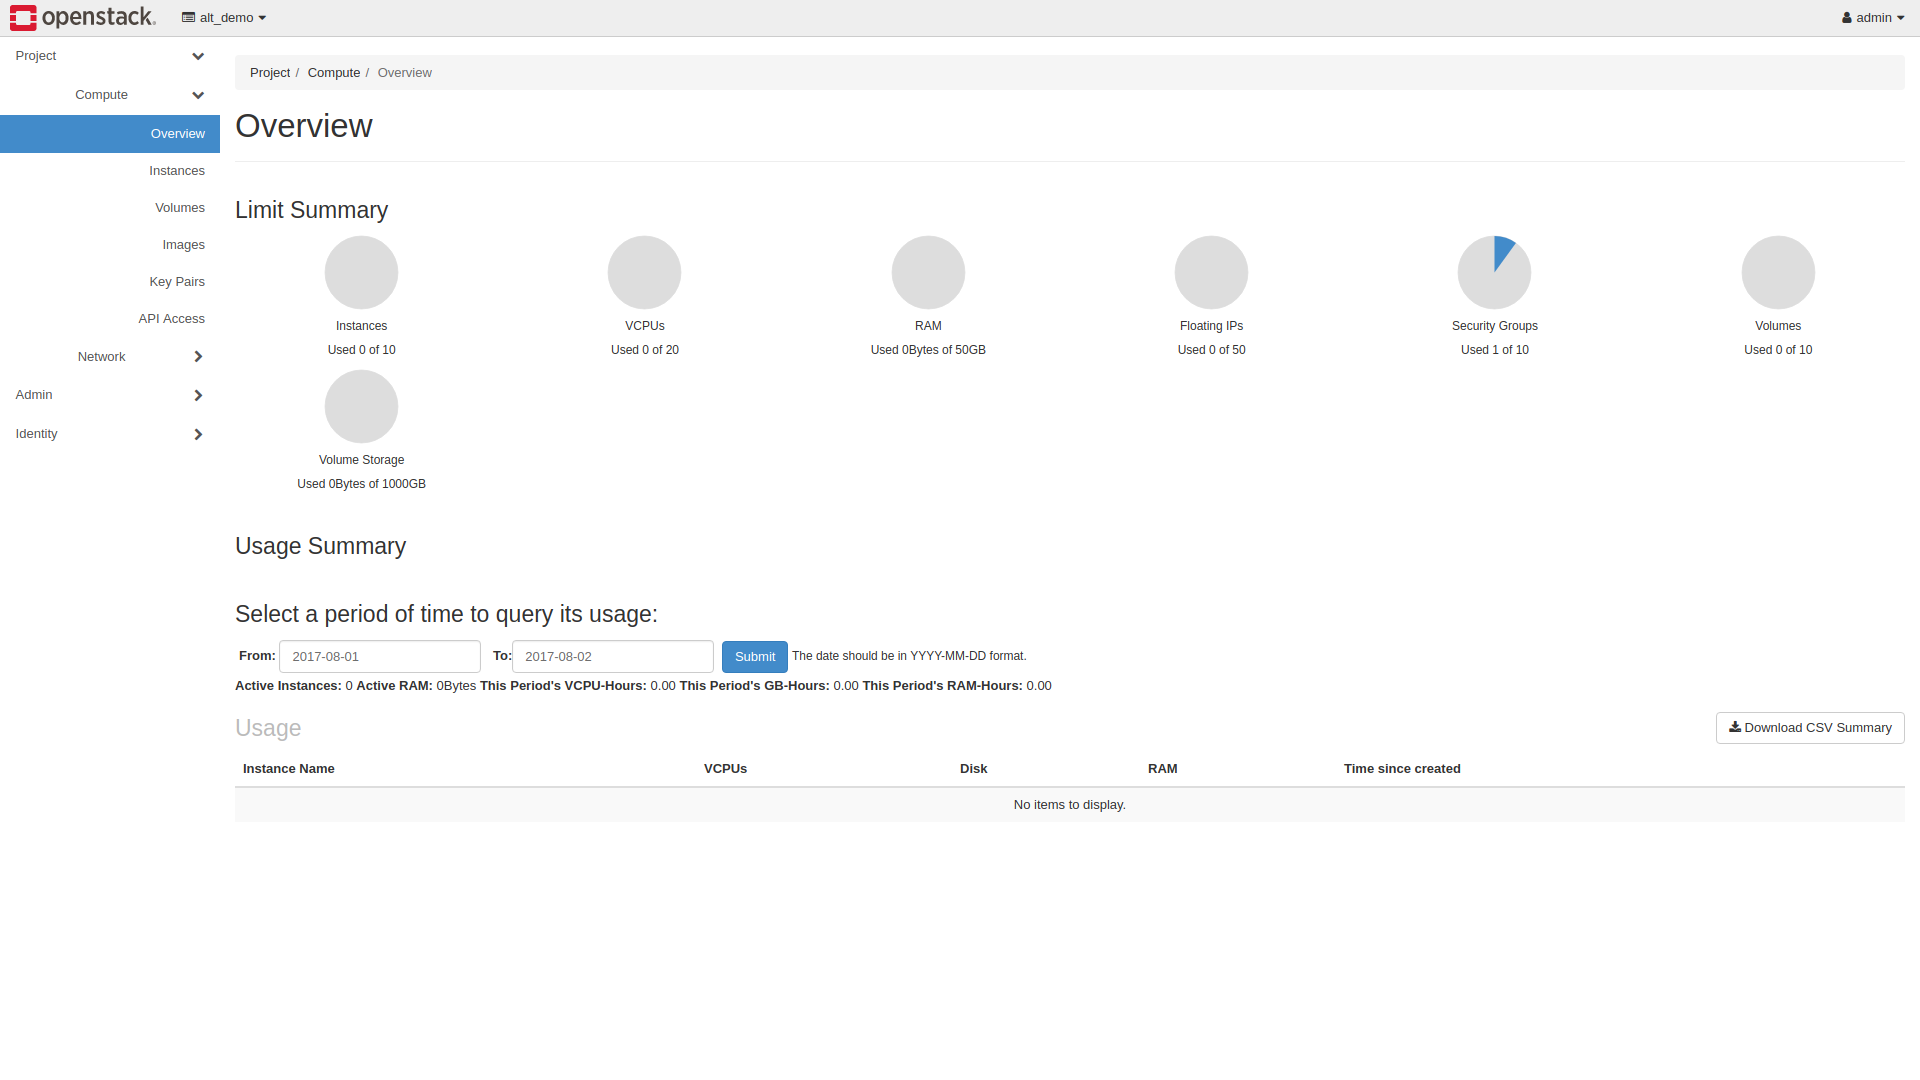
\includegraphics[width=\textwidth]{graphics/devstack/01_Overview}
\end{figure}

\begin{minipage}{\textwidth}
Hier ist eine kurze Beschreibung der Punkte:
\begin{itemize}
 \item Instances - die aktuell geladenen Instanzen, diese werden unten genauer beschrieben
 \item VCPUs - die virtuellen CPUs, Instanzen werden für die Ausführung auf diese aufgeteilt
 \item RAM - der RAM wird ebenso wie die CPUs unter den Instanzen aufgeteilt
 \item Floating IPs - diese können Instanzen zugewiesen werden, damit diese von außerhalb der Cloud erreichbar sind
 \item Security Groups - Die security groups bieten die Möglichkeit ip-Filter für ein Projekt anzulegen. Jedes Projekt erhält nach dem Erstellen standardmäßig einen Filter der alle IPs blockiert. "Security groups are sets of IP filter rules that are applied to an instance’s networking." \url{https://www.mirantis.com/openstack-portal/express-openstack-portal/manage-openstack-security-groups-via-horizon/}
 \item Volumes - Diese verwalten den verfügbaren Festplattenspeicher. Es können Volumen mit einer bestimmten Speicherkapazität erstellt werden und Instanzen zugewiesen werden. Jede Instanz benötigt mindestens ein Volume.
 \item Volume Storage - dieses Diagram bietet einen Überblick über den Speicherplatz den die Volumes belegen.
\end{itemize}
\end{minipage}

\subparagraph{Instances}

\begin{figure}[htbp]
\centering
\caption{Überblick über das Projekt}
\label{fig:devstack:overview}
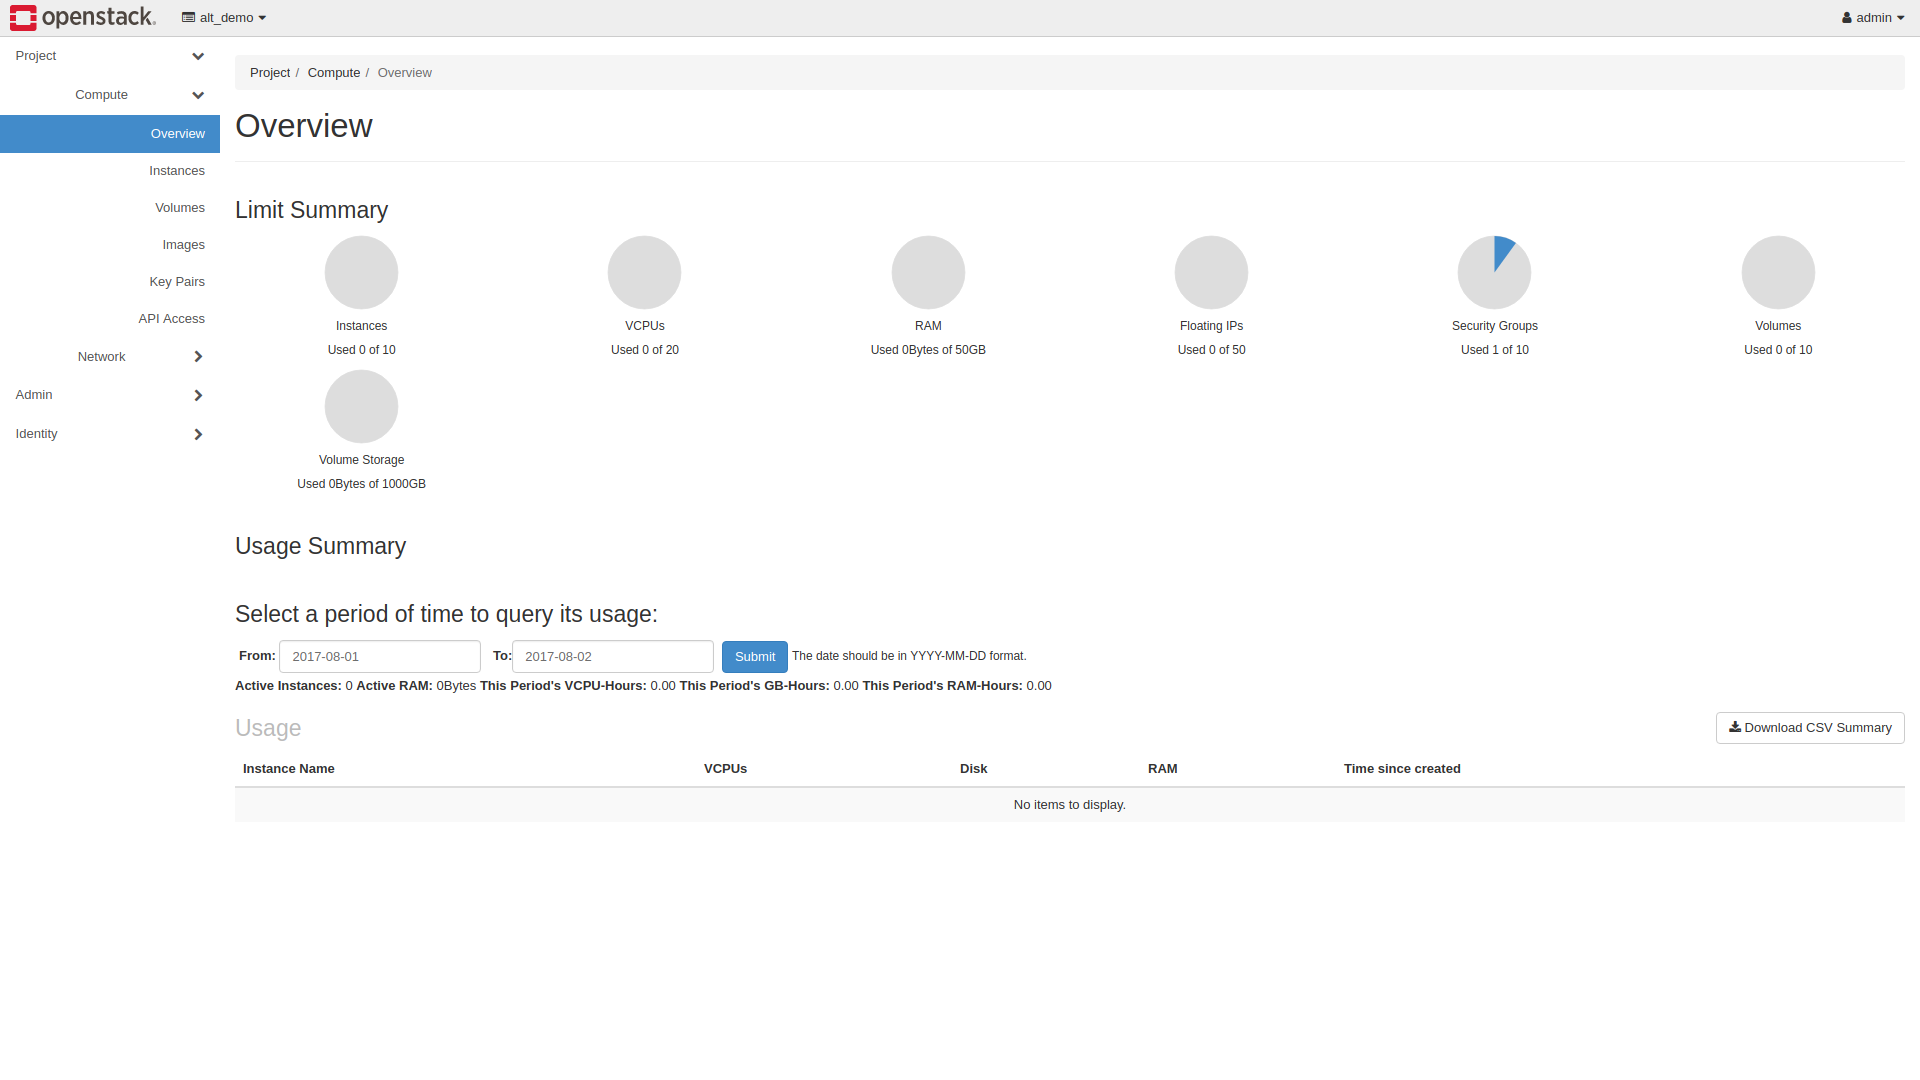
\includegraphics[width=\textwidth, trim={0 5cm 0 0}, clip]{graphics/devstack/01_Overview}
\end{figure}

\subparagraph{Volumes}

Von hier können die Volumes gesteuert werden.
Es gibt einen Überblick über alle bestehenden Instanzen.
In der Abbildung \ref{fig:devstack:volumes} existiert ein Volume.
Es hat den Namen 'New Volume' und ist 4GB groß.

\begin{figure}[htbp]
\centering
\caption{Volumes des Projekts}
\label{fig:devstack:volumes}
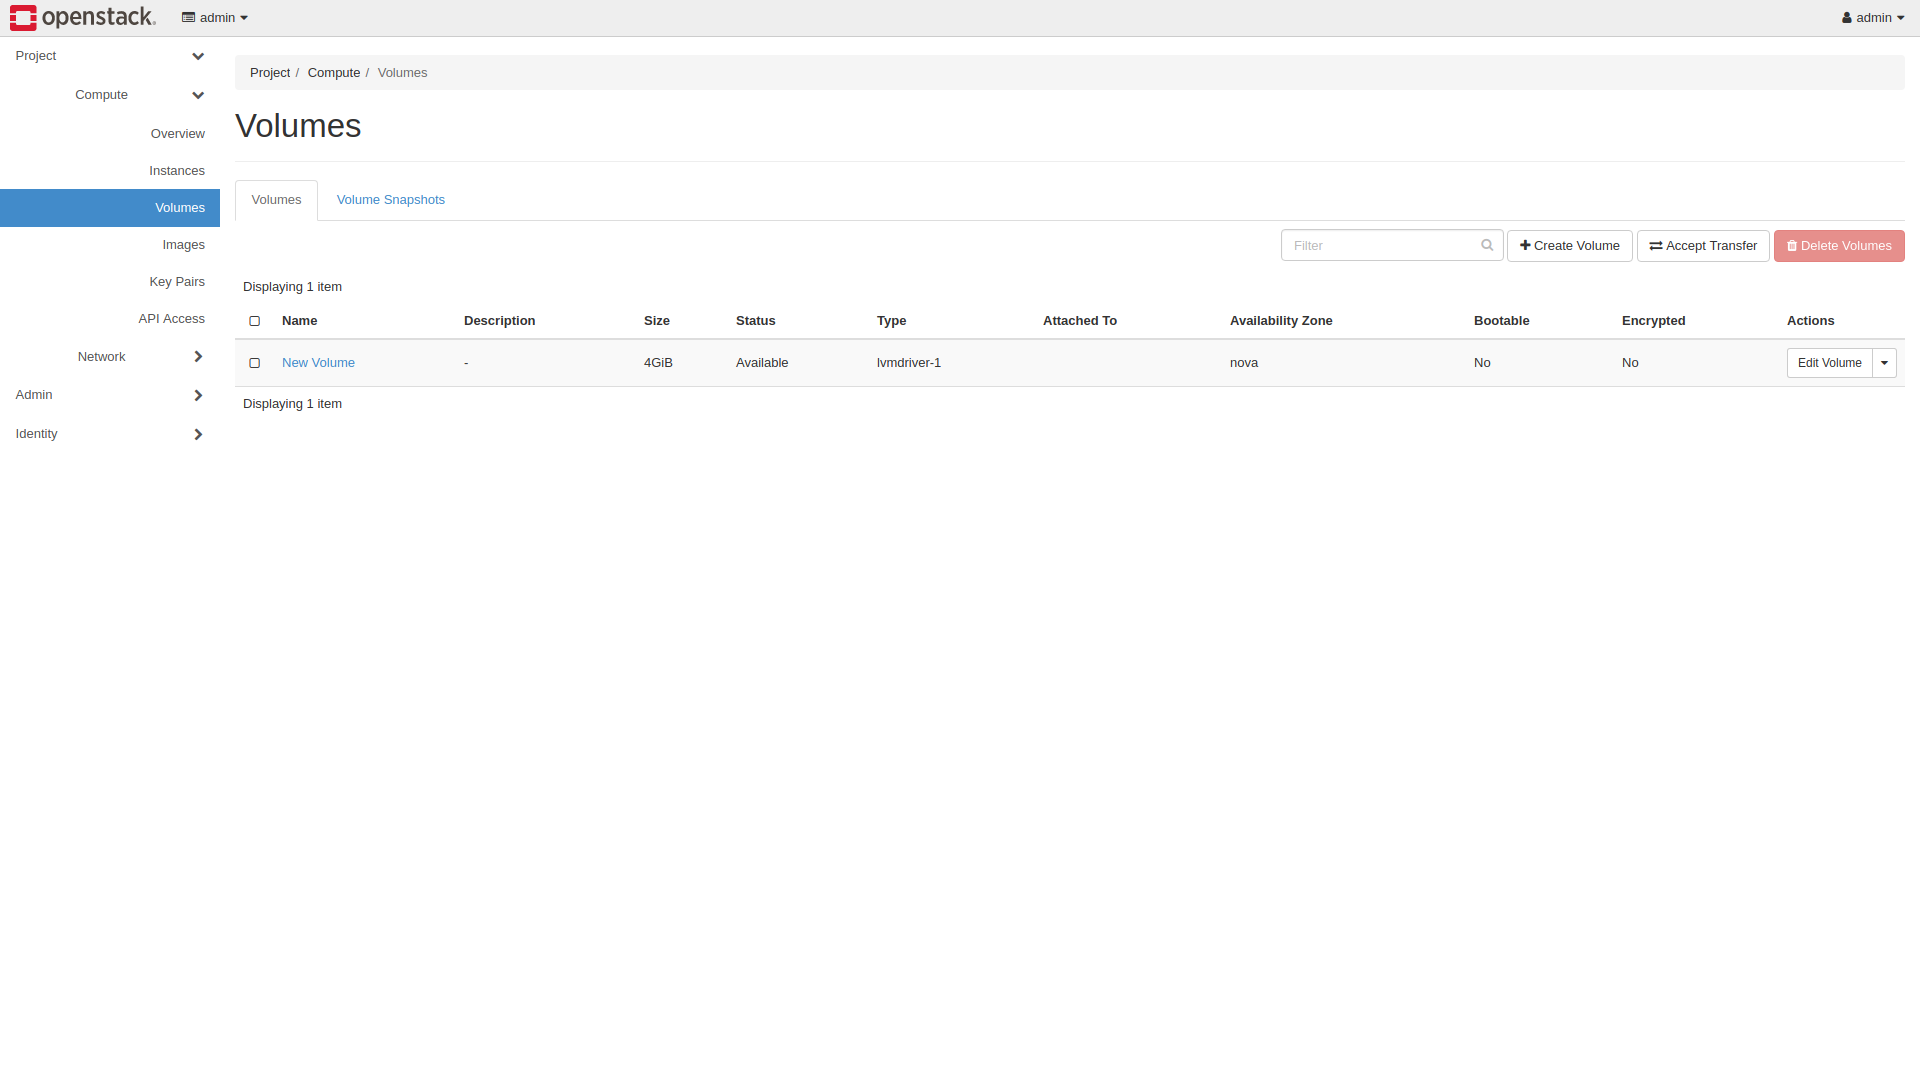
\includegraphics[width=\textwidth, trim={0 17cm 0 0}, clip]{graphics/devstack/14_AddedVolume}
\end{figure}

\subparagraph{Images}

\begin{figure}[htbp]
\centering
\caption{Volumes des Projekts}
\label{fig:devstack:volumes}
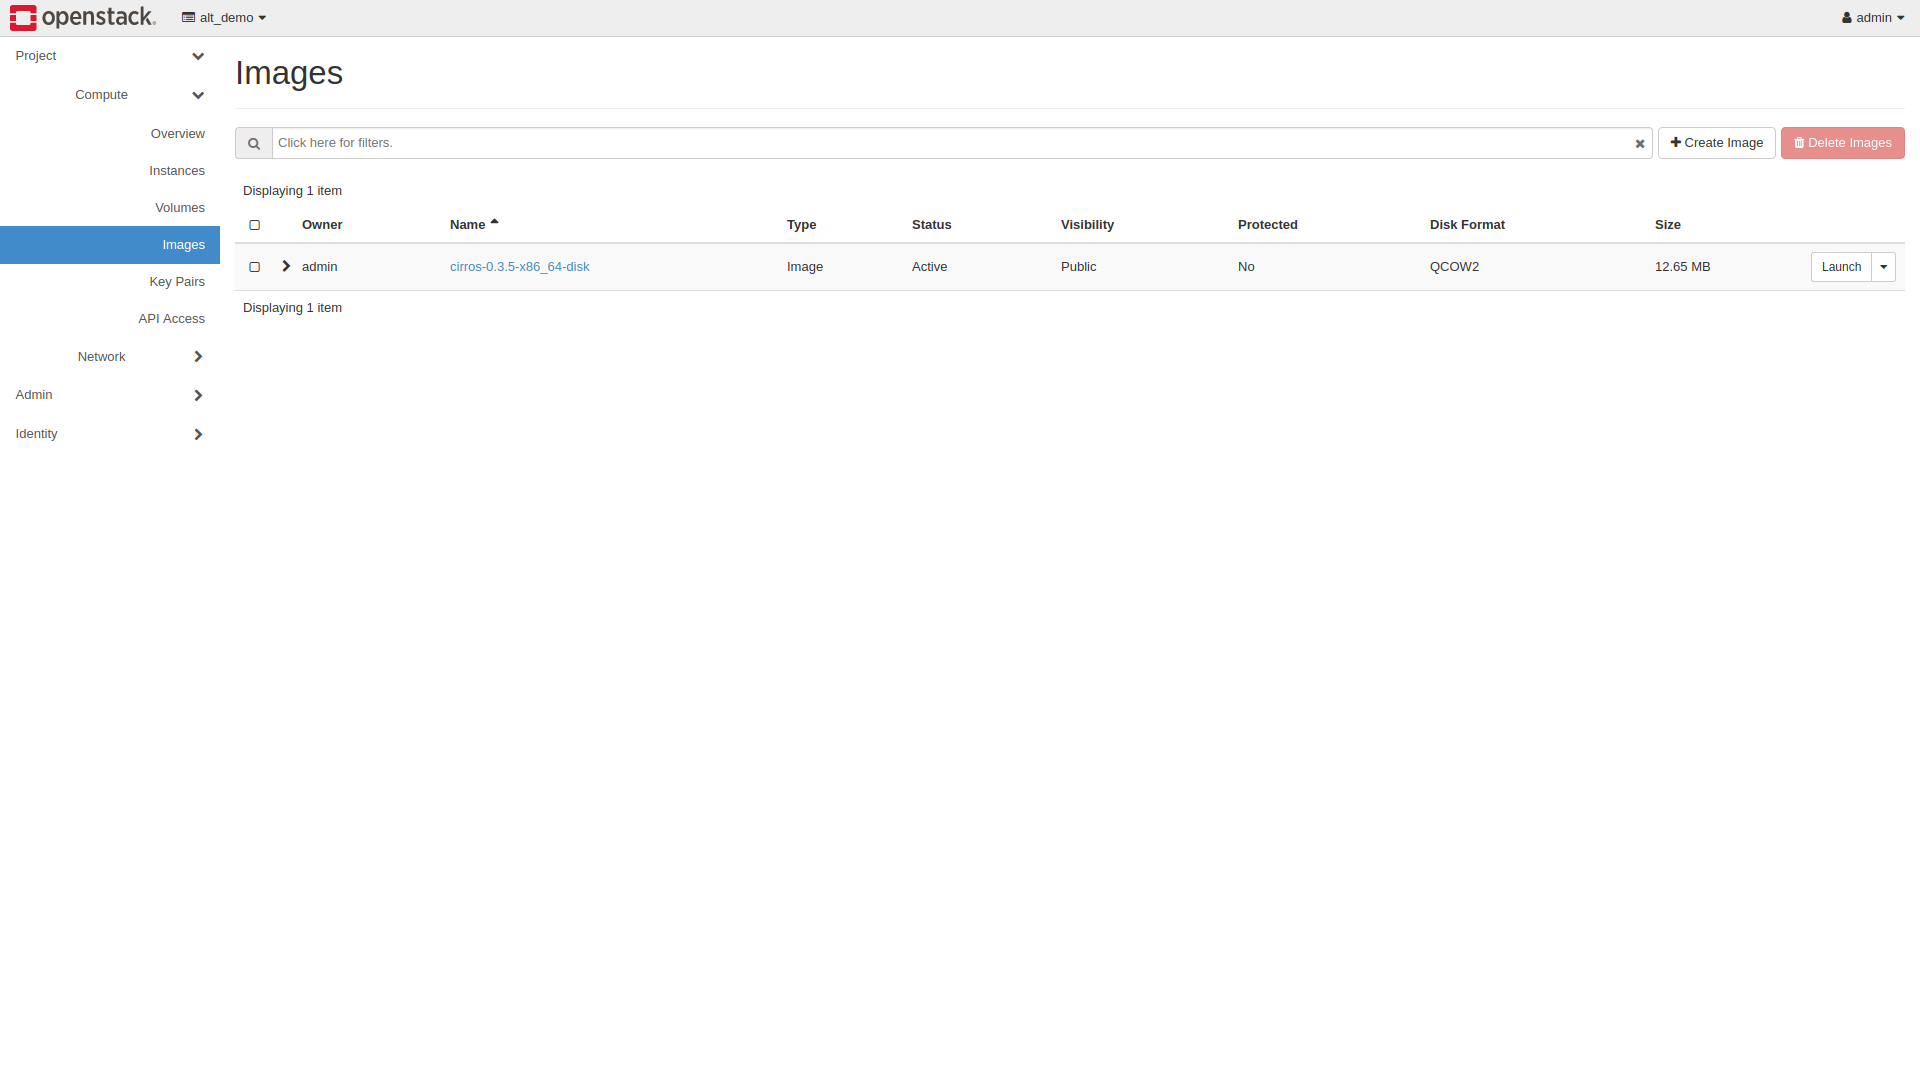
\includegraphics[width=\textwidth, trim={0 17cm 0 0}, clip]{graphics/devstack/02_Images}
\end{figure}

\subparagraph{Key Pairs}

\begin{figure}[htbp]
\centering
\caption{Volumes des Projekts}
\label{fig:devstack:volumes}
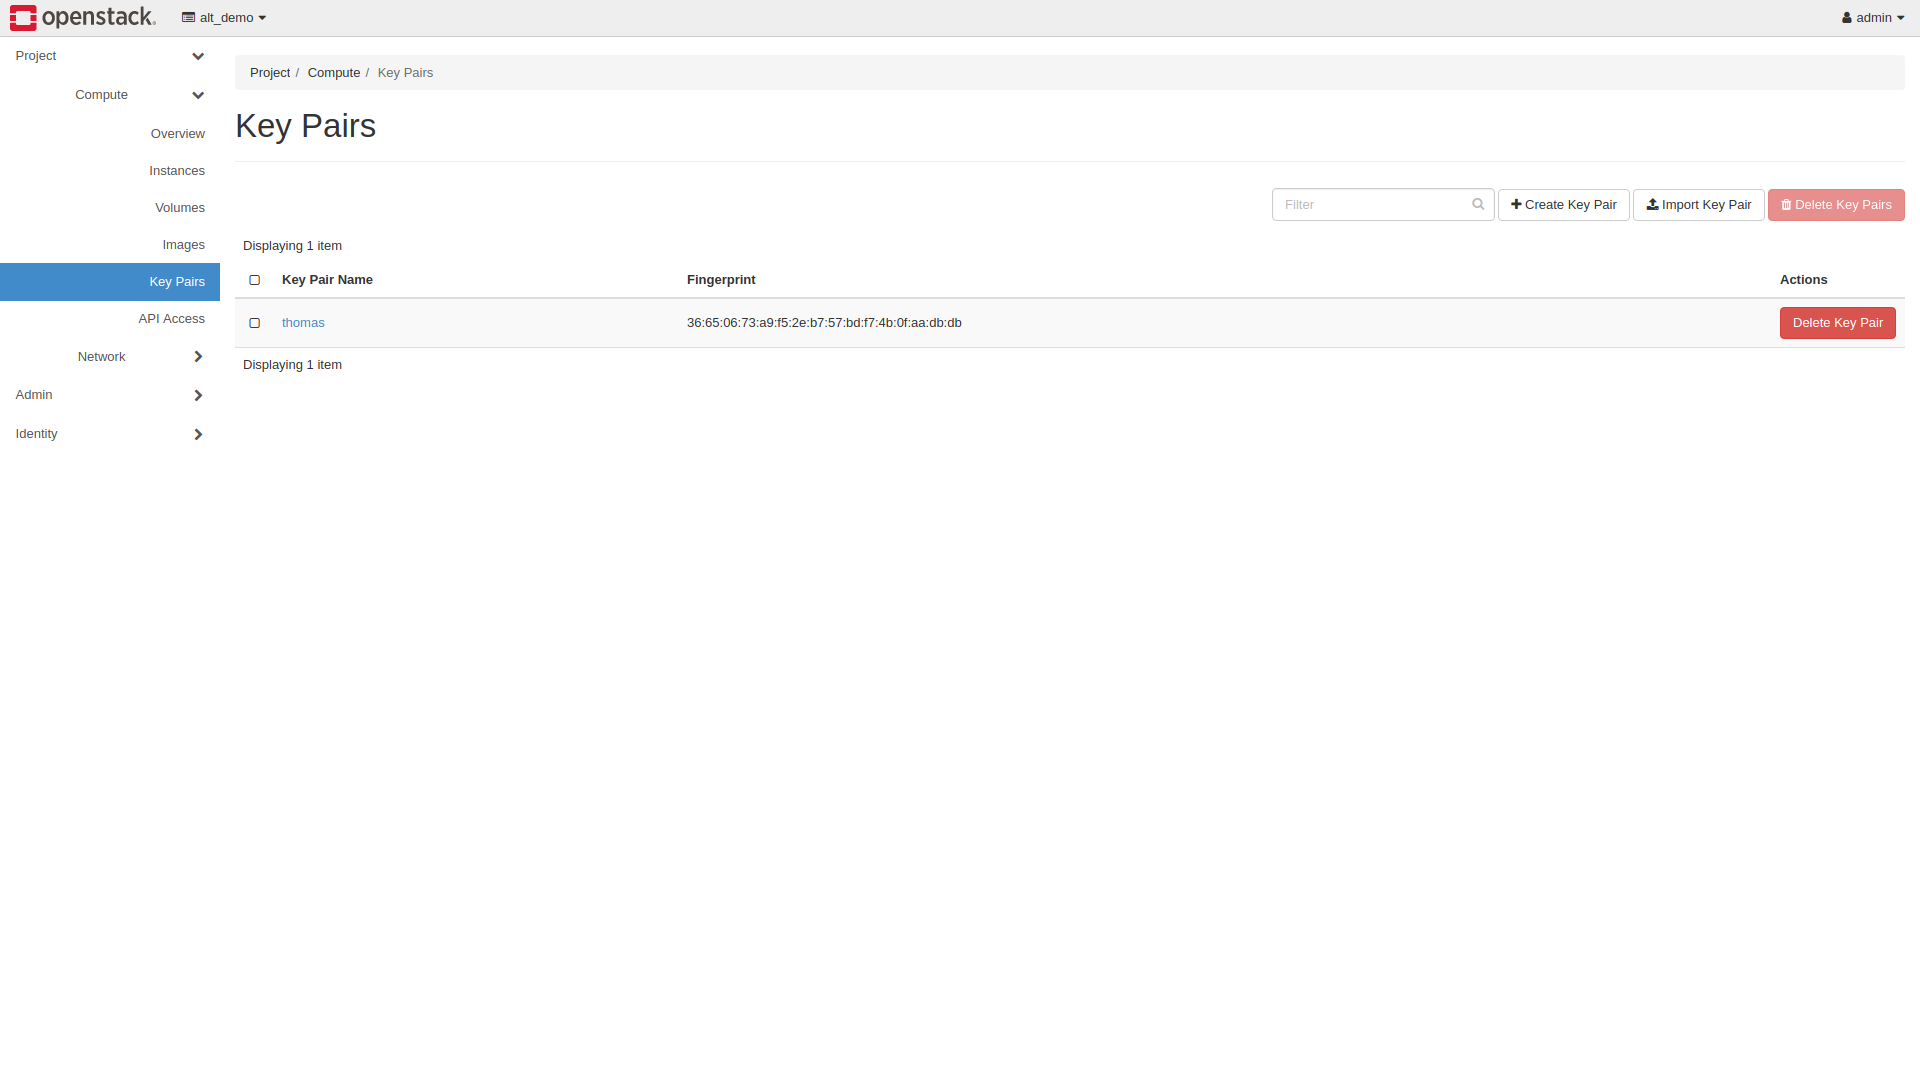
\includegraphics[width=\textwidth, trim={0 17cm 0 0}, clip]{graphics/devstack/03_KeyPairs}
\end{figure}

\subparagraph{API Access}

\begin{figure}[htbp]
\centering
\caption{API Zugriff auf das Projekts}
\label{fig:devstack:volumes}
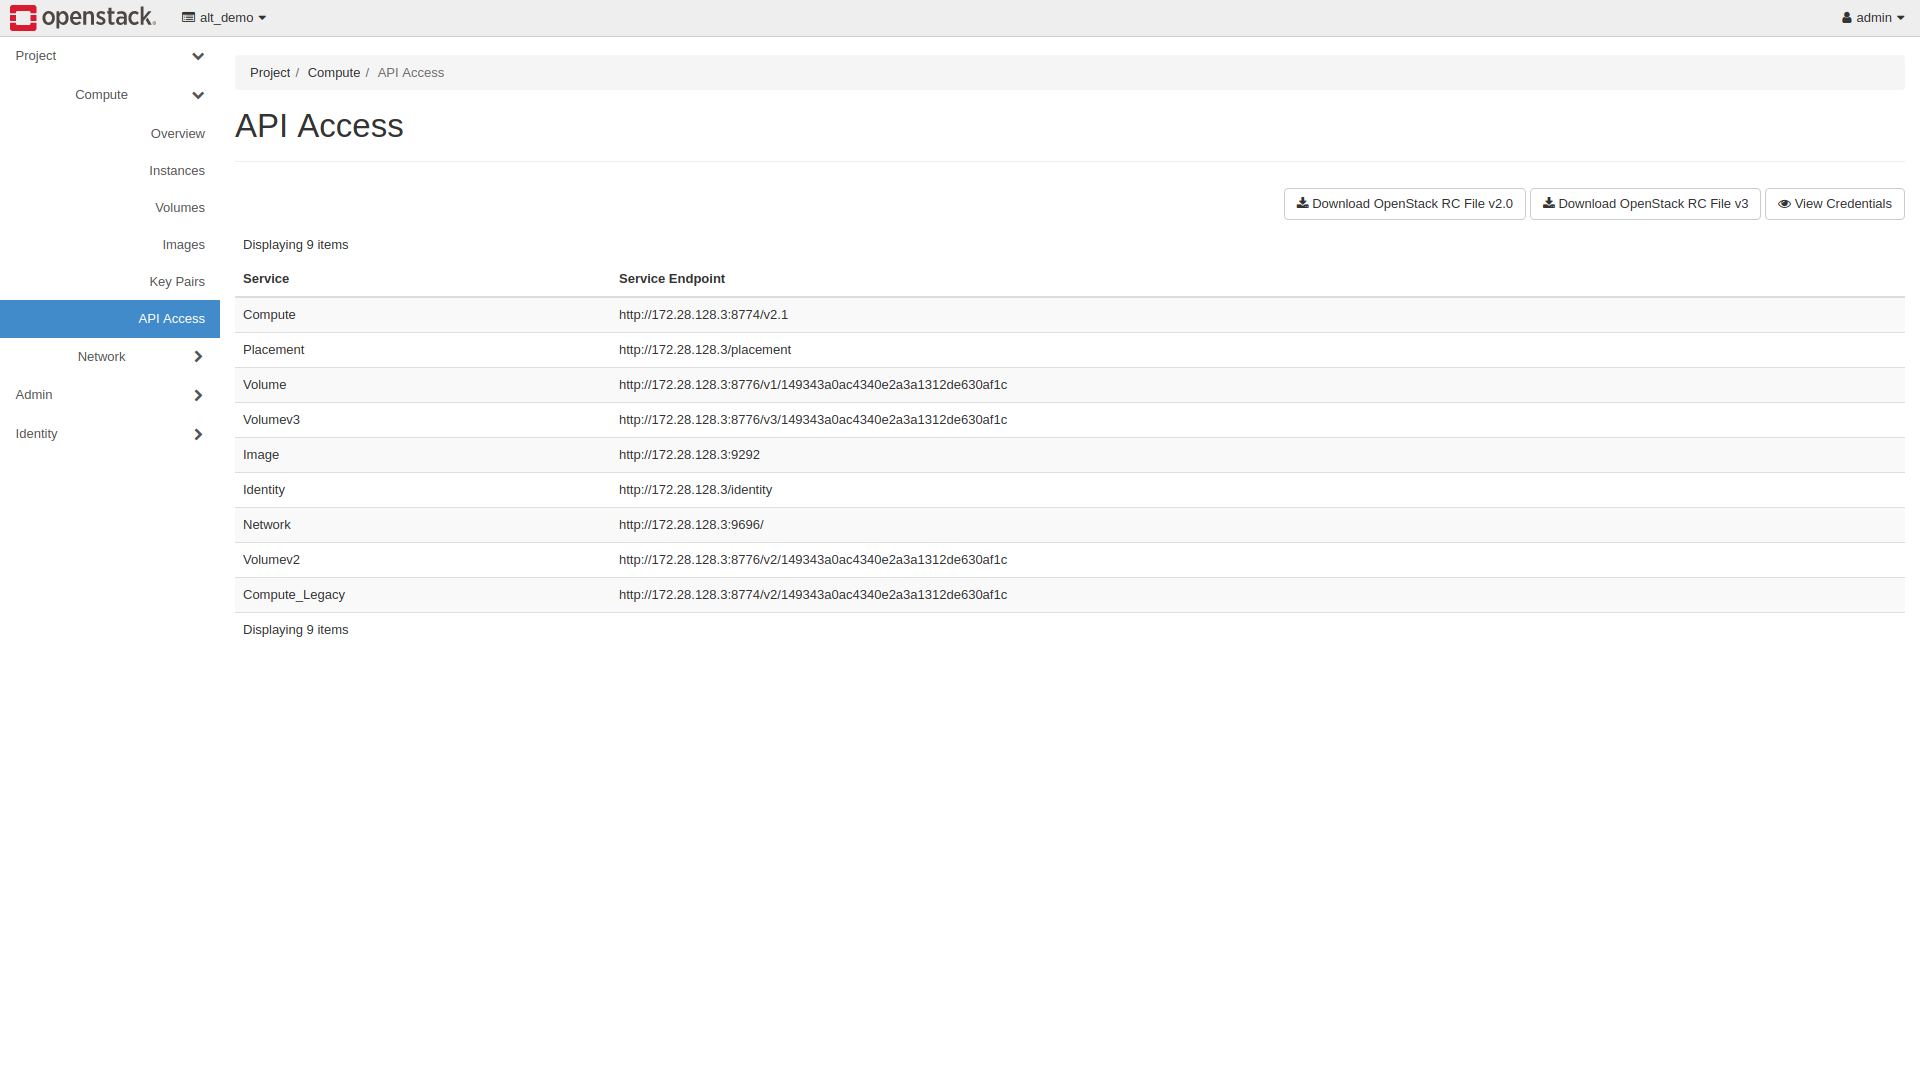
\includegraphics[width=\textwidth, trim={0 10cm 0 0}, clip]{graphics/devstack/04_ApiAccess}
\end{figure}

\paragraph{Workflow zum Erstellen einer Instanz}

\todo{evtl. anhand eines Workflow}

\paragraph{Vorbereitung für die Installation}

\subparagraph{Ubuntu 16.04 in Vagrant aufsetzen}

\begin{enumerate}
 \item \begin{verbatim}vagrant init bento/ubuntu-16.04\end{verbatim}
 \item Vagrantfile anpassen. Es sollten mindestens 4GB RAM zugewiesen werden, damit OpenStack performant läuft.\\
\begin{minipage}{\textwidth}
\begin{lstlisting}[frame=single,caption=Installation Ubuntu 16.04 in Vagrant]
Vagrant.configure(2) do |config|
  config.vm.box = "bento/ubuntu-16.04"
  config.vm.network "private_network", type: "dhcp"
 
  config.vm.provider "virtualbox" do |v|
    v.memory = 4096
  end
end
\end{lstlisting}
\end{minipage}
 \item \begin{verbatim}vagrant up\end{verbatim}
 \item \begin{verbatim}vagrant ssh\end{verbatim}
\end{enumerate}
 
\paragraph{Installation}
 
\subparagraph{Devstack installieren}
  
\begin{enumerate}
 \item \begin{verbatim}git clone https://git.openstack.org/openstack-dev/devstack \end{verbatim}
 \item  \begin{verbatim}cd devstack\end{verbatim}
 \item Bei Bedarf zu einem (älteren) stable release wechseln: \begin{verbatim}git checkout stable/ocata\end{verbatim} oder \begin{verbatim}git checkout stable/mitaka\end{verbatim} Die master-branch kann auch genutzt werden.
 \item \begin{verbatim}ifconfig enp0s8 | grep addr\end{verbatim}
 \item \begin{verbatim}inet addr kopieren\end{verbatim}
 \item \begin{verbatim}cp samples/local.conf .\end{verbatim}
 \item \begin{verbatim}HOST_IP="xxx.xxx.xxx.xxx"\end{verbatim}
 \item \begin{verbatim}echo "HOST_IP=${HOST_IP}" >> local.conf\end{verbatim}
 \item Es muss ein user mit sudo-rechten (ohne passwort) existieren, der nicht root ist. Der Standarduser vagrant ist dafür geeignet.
 \item \begin{verbatim}./stack.sh\end{verbatim}
\end{enumerate}

Am Ende der erfolgreichen Installation erscheint die folgende Ausgabe in etwa so.
Von hier können die nötigen Informationen für das weitere Vorgehen entnommen werden.

\begin{minipage}{\textwidth}
\begin{lstlisting}[frame=single,caption=Ausgabe von DevStack]
=========================
DevStack Component Timing
=========================
Total runtime         3644

run_process            87
test_with_retry         7
apt-get-update         12
pip_install           881
restart_apache_server  20
wait_for_service       61
git_timed             355
apt-get               457
=========================



This is your host IP address: 172.28.128.3
This is your host IPv6 address: ::1
Horizon is now available at http://172.28.128.3/dashboard
Keystone is serving at http://172.28.128.3/identity/
The default users are: admin and demo
The password: nomoresecret
\end{lstlisting}
\end{minipage}

\paragraph{Starten}

\subparagraph{Openstack (Horizon) starten}

Die folgenden Informationen sind abhängig von der Konfiguration.
Für dieses Beispiel sind folgende Daten notwendig.

\begin{enumerate}
 \item \url{http://172.28.128.3/dashboard} in einem Browser öffnen
 \item Benutzername admin oder demo
 \item Password nomoresecret
\end{enumerate}

\subparagraph{Reboot}

\url{https://ask.openstack.org/en/question/5423/rebooting-with-devstack/}
Wenn die Vagrantbox herunter gefahren wurde muss devstack nach einem erneuten Start ebenfalls neu gestartet werden.
Ansonsten können die verschiedenen Services nicht genutzt werden.
Das Webfrontend Horizon kann in diesem Fall keinerlei Ressourcen laden.
Zum erneuten Erstellen der openstack Umgebung können die folgenden Befehle genutzt werden.

\begin{verbatim}
 ./unstack.sh
 ./stack.sh
\end{verbatim}

Bei einem erneuten Ausführen von stack.sh würden jedoch alle Datenbanken neu erstellt werden.
Das würde zu einem kompletten Datenverlust führen.
Dies ist aber nicht in jedem Fall gewünscht.
Dafür steht eine screen-Konfiguration bereit mit der die notwendigen Services gestartet werden können.

\url{http://stackoverflow.com/questions/36268822/no-rejoin-stack-sh-script-in-my-setup}

\begin{verbatim}
 screen -c stack-screenrc
\end{verbatim}

So kann eine bestehende openstack-Konfiguration auch nach einem Neustart weiter genutzt werden.

\paragraph{SSH-Verbindung zur Cloud}

http://openstack-cloud-mylearning.blogspot.de/2015/02/openstack-how-to-access-vm-using-ssh.html

\newpage













\section{Gegenüberstellung verfügbarer Werkzeuge und Varianten}
\todo{vergleiche kapitel ausarbeiten}

\subsection{'private' und 'public' Cloud}

\begin{itemize}
 \item gibt es open source cloud systeme? welche?
 \item welche public clouds gibt es (zB aws, windows azure, adobe creative)
 \item was sind unterschiede (neben dem access, zB performance?)
\end{itemize}

\subsection{Technologie}

\todo{tabelle/vergleiche zwischen technologien: rpc,socket,service etc}

\begin{itemize}
 \item welche Werkzeuge für die kommunikation zwischen client und cloud
 \item rpc, socket, service ...
 \item abwägen zwischen performance, aufwand ...
 \item welche framework könnten genutzt werden
\end{itemize}

\subsection{Cloudtyp}

wird evtl schon teilweise in abschnitt 1 (allgemeines zur cloud) abgedeckt

\begin{itemize}
 \item Infrastructure as a Service (IaaS)
 \item Platform as a Service (PaaS)
 \item Software as a Service (SaaS)
 \item aber entscheidend: wie eignen sich diese typen für `unsere` Implementierung
\end{itemize}

\subsection{Sprache}

\begin{itemize}
 \item hardware-nah: C/C++ (bessere performance)
 \item vs netzwerknah: (bessere möglichkeiten die kommunikation zu Implementieren)
 \item kann eine hybridform eingsetzt werden? 
 zB (micro-)service: bib in c kommuniziert mit client-backend in php, dieses führt die calls zum server aus
\end{itemize}

\subsection{Vergleich ausgewählter Cloudsysteme in einer Tabelle}

anhand relevanter (für das Projekt) Eigenschaften

\begin{table}[]
\centering
\caption{Vergleich von Cloudanbietern}
\label{my-label}
\renewcommand{\arraystretch}{1.5}
\begin{tabular}{llllll}
\hline
Cloudsystem & private & public & PaaS & ... & ...\\
\hline
Openstack & \mycheckbox & ... & ... & ... & ...\\
Apache CS & \mycheckbox & ... & ... & ... & ...\\
Amazon AWS & \myuncheckbox & ... & \mycheckbox & ... &  ...\\
\hline
\end{tabular}
\end{table}

\newpage













\section{Auswertung der Vergleiche und Auswahl der Werkzeuge}

Vergleiche verschiedener Technologien und Werkzeuge.
Auswahl für den Einsatz bei der Implementierung.

\subsection{gRPC} \url{http://www.grpc.io/}

Googles open source RPC framework.
Dokumentation: \url{http://www.grpc.io/docs/}.

\paragraph{Installation}

Installiere vagrant ubuntu 16.04.
Setup von gRPC nach der Installation:

\begin{lstlisting}[frame=single,caption=Installiere vagrant ubuntu 16.04]
cd /vagrant
sudo apt-get install build-essential autoconf libtool
sudo apt-get install libgflags-dev libgtest-dev
sudo apt-get install clang libc++-dev
git clone -b $(curl -L http://grpc.io/release) \\
https://github.com/grpc/grpc
cd grpc
git submodule update --init
make && sudo make install
cd third_party/protobuf
sudo apt-get install unzip
./autogen.sh
./configure
make && sudo make install
cd -
cd examples/cpp/helloworld/
sudo apt-get install pkg-config
make
\end{lstlisting}

\paragraph{kurze Einführung}

\todo{grpc genauer beschreiben (auch protobuf)}

Benutzt Protobuf zum erstellen von Services und Nachrichtenobjekten (stubs).
Offizieller support für C++ vorhanden.
Implementierung für c vorhanden \url{https://github.com/protobuf-c/protobuf-c}.
Das Basisframework von gRPC ist ebenfalls in nativem C geschrieben.
Die Highlevel-Framework-API ist jedoch nicht in C verfügbar.

Da die Definitionen der stubs nicht sprachgebunden erfolgen ist eine (spätere) Umstellung auf eine andere Sprache einfacher.
Es müssen die stubs für die neue Sprache lediglich aus den gleichen Definitionen neu generiert werden.

\begin{lstlisting}[frame=single,caption=Beispiel grpc]
package helloworld;

// The greeting service definition.
service Greeter {
  // Sends a greeting
  rpc SayHello (HelloRequest) returns (HelloReply) {}
}

// The request message containing the user's name.
message HelloRequest {
  string name = 1;
}

// The response message containing the greetings
message HelloReply {
  string message = 1;
}
\end{lstlisting}

\paragraph{Überblick Funktionsumfang}

Ein definierter Service steht nach dem generieren der Implementierung in der gewünschten Sprache als Interface bereit.
Dieses kann alternativ auch als AsyncService implementiert werden.

\begin{lstlisting}[frame=single,caption=grpc Service Definition]
//synchron
class X : public Greeter::Service {}
//oder asynchron
class X : public Greeter::AsyncService {}
\end{lstlisting}

Listen von Request- oder Responseobjekten können in Form eines Streams übertragen werden.

\begin{lstlisting}[frame=single,caption=grpc Funktion Definition]
rpc ListFeatures(Rectangle) returns (stream Feature) {}
\end{lstlisting}

\subsection{Ressourcen}

\begin{itemize}
 \item HPC in der Cloud \url{http://grids.ucs.indiana.edu/ptliupages/publications/cloud_handbook_final-with-diagrams.pdf}
\end{itemize}

\subsection{Roadmap Implementierung}

\todo{roadmap checken/erweitern/abhaken}

\paragraph{Was muss zwischen Client und Server übertragen werden:}

Anzahl der calls zwischen Client und Server sollte so gering wie möglich gehalten werden.
Der Aufbau der Datenstrukturen sollte daher komplett innerhalb des Clients passieren.
Sobald alle Eingabedaten erstellt sind muss ein Solver aufgerufen werden.
Die Solver sollten auf dem Server ausgeführt werden.

\subparagraph{(später:)}

Eventuell kann sogar der Aufwand der Berechnung abgeschätzt werden.
Somit könnten einfache Berechnungen innerhalb des Client ausgeführt werden.
Lediglich komplexe Berechnungen an den Server übermittelt werden.

\subparagraph{Fazit}

1. Möglichkeit:
Es müssen (alle) HYPRE-Datentypen übertragen werden können.
Dazu muss ein Mapper existieren.
Dieser sollte die Datenstrukturen in ein Datenformat umwandeln welches übertragen werden kann (json).
Er muss außerdem die übertragbaren Daten wieder in die Datenstrukturen zurück umwandeln können.

2. Möglichkeit:
Alle Eingabeparameter und Funktionsaufrufe werden gesammelt.
Auf Seite des Servers werden diese nacheinander ausgeführt um die Datenstrukturen zu bilden.
Danach wird der Solver ausgeführt.
Am Ende die lediglich die Antwort umgewandelt und übertragen.

\paragraph{Client}

\subparagraph{Anforderungen}

Bibliothek.
Alle HYPRE-Calls implementieren die einen solver ausführen.
Statt der direkten Ausführung müssen die Input-Daten an den Server übertragen werden.
Außerdem muss der Call-Name übertragen werden.
Nach Ausführung auf dem Server muss die Antwort wiederum in die entsprechenden Datentypen umgewandelt werden.

\subparagraph{Kernmodule}

Einige HYPRE-Methoden überschreiben.
Mapping HYPRE-Datentypen zu JSON.
Mapping JSON zu HYPRE-Datentypen.
Webservices implementieren für Komunikation mit dem Server.

\newpage













\section{Verteilten Ausführung von HYPRE}

\newpage













\section{Zukünftige, weiterführende Arbeiten}

\todo{eventuell werden Teile von hier in die aktuelle Arbeit verschoben}

\begin{itemize}
 \item Skalierbarkeit der Cloud (einsetzen)
 \item Benchmarking lokal vs. remote HPC vs. cloud vs. ...
 \item daraus ableiten: Vorteile der Auslagerung:
  \begin{itemize}
    \item Performance
    \item Speicher
    \item Lösbarkeit (nur remote überhaupt lösbar)
  \end{itemize}
 \item Beispiel in nutzbares Framework umwandeln
 \item Beispiel nicht nur lokal sonder auch in Cloudumgebung
 \item auf remote Seite (effektiv) parallelisieren
\end{itemize}

\newpage








\bibliographystyle{apacite}
\bibliography{cites}

\newpage










\appendix
\section{\\HYPRE}
\subsection{HYPRE Example 5}
\begin{lstlisting}
/*
   Example 5

   Interface:    Linear-Algebraic (IJ)

   Compile with: make ex5

   Sample run:   mpirun -np 4 ex5

   Description:  This example solves the 2-D Laplacian problem with zero boundary
                 conditions on an n x n grid.  The number of unknowns is N=n^2.
                 The standard 5-point stencil is used, and we solve for the
                 interior nodes only.

                 This example solves the same problem as Example 3.  Available
                 solvers are AMG, PCG, and PCG with AMG or Parasails
                 preconditioners.  */

#include <math.h>
#include "_hypre_utilities.h"
#include "HYPRE_krylov.h"
#include "HYPRE.h"
#include "HYPRE_parcsr_ls.h"

#include "vis.c"

int hypre_FlexGMRESModifyPCAMGExample(void *precond_data, int iterations,
                                      double rel_residual_norm);


int main (int argc, char *argv[])
{
   int i;
   int myid, num_procs;
   int N, n;

   int ilower, iupper;
   int local_size, extra;

   int solver_id;
   int vis, print_system;

   double h, h2;

   HYPRE_IJMatrix A;
   HYPRE_ParCSRMatrix parcsr_A;
   HYPRE_IJVector b;
   HYPRE_ParVector par_b;
   HYPRE_IJVector x;
   HYPRE_ParVector par_x;

   HYPRE_Solver solver, precond;

   /* Initialize MPI */
   MPI_Init(&argc, &argv);
   MPI_Comm_rank(MPI_COMM_WORLD, &myid);
   MPI_Comm_size(MPI_COMM_WORLD, &num_procs);

   /* Default problem parameters */
   n = 33;
   solver_id = 0;
   vis = 0;
   print_system = 0;


   /* Parse command line */
   {
      int arg_index = 0;
      int print_usage = 0;

      while (arg_index < argc)
      {
         if ( strcmp(argv[arg_index], "-n") == 0 )
         {
            arg_index++;
            n = atoi(argv[arg_index++]);
         }
         else if ( strcmp(argv[arg_index], "-solver") == 0 )
         {
            arg_index++;
            solver_id = atoi(argv[arg_index++]);
         }
         else if ( strcmp(argv[arg_index], "-vis") == 0 )
         {
            arg_index++;
            vis = 1;
         }
         else if ( strcmp(argv[arg_index], "-print_system") == 0 )
         {
            arg_index++;
            print_system = 1;
         }
         else if ( strcmp(argv[arg_index], "-help") == 0 )
         {
            print_usage = 1;
            break;
         }
         else
         {
            arg_index++;
         }
      }

      if ((print_usage) && (myid == 0))
      {
         printf("\n");
         printf("Usage: %s [<options>]\n", argv[0]);
         printf("\n");
         printf("  -n <n>              : problem size in each direction (default: 33)\n");
         printf("  -solver <ID>        : solver ID\n");
         printf("                        0  - AMG (default) \n");
         printf("                        1  - AMG-PCG\n");
         printf("                        8  - ParaSails-PCG\n");
         printf("                        50 - PCG\n");
         printf("                        61 - AMG-FlexGMRES\n");
         printf("  -vis                : save the solution for GLVis visualization\n");
         printf("  -print_system       : print the matrix and rhs\n");
         printf("\n");
      }

      if (print_usage)
      {
         MPI_Finalize();
         return (0);
      }
   }

   /* Preliminaries: want at least one processor per row */
   if (n*n < num_procs) n = sqrt(num_procs) + 1;
   N = n*n; /* global number of rows */
   h = 1.0/(n+1); /* mesh size*/
   h2 = h*h;

   /* Each processor knows only of its own rows - the range is denoted by ilower
      and upper.  Here we partition the rows. We account for the fact that
      N may not divide evenly by the number of processors. */
   local_size = N/num_procs;
   extra = N - local_size*num_procs;

   ilower = local_size*myid;
   ilower += hypre_min(myid, extra);

   iupper = local_size*(myid+1);
   iupper += hypre_min(myid+1, extra);
   iupper = iupper - 1;

   /* How many rows do I have? */
   local_size = iupper - ilower + 1;

   /* Create the matrix.
      Note that this is a square matrix, so we indicate the row partition
      size twice (since number of rows = number of cols) */
   HYPRE_IJMatrixCreate(MPI_COMM_WORLD, ilower, iupper, ilower, iupper, &A);

   /* Choose a parallel csr format storage (see the User's Manual) */
   HYPRE_IJMatrixSetObjectType(A, HYPRE_PARCSR);

   /* Initialize before setting coefficients */
   HYPRE_IJMatrixInitialize(A);

   /* Now go through my local rows and set the matrix entries.
      Each row has at most 5 entries. For example, if n=3:

      A = [M -I 0; -I M -I; 0 -I M]
      M = [4 -1 0; -1 4 -1; 0 -1 4]

      Note that here we are setting one row at a time, though
      one could set all the rows together (see the User's Manual).
   */
   {
      int nnz;
      double values[5];
      int cols[5];

      for (i = ilower; i <= iupper; i++)
      {
         nnz = 0;

         /* The left identity block:position i-n */
         if ((i-n)>=0)
         {
            cols[nnz] = i-n;
            values[nnz] = -1.0;
            nnz++;
         }

         /* The left -1: position i-1 */
         if (i%n)
         {
            cols[nnz] = i-1;
            values[nnz] = -1.0;
            nnz++;
         }

         /* Set the diagonal: position i */
         cols[nnz] = i;
         values[nnz] = 4.0;
         nnz++;

         /* The right -1: position i+1 */
         if ((i+1)%n)
         {
            cols[nnz] = i+1;
            values[nnz] = -1.0;
            nnz++;
         }

         /* The right identity block:position i+n */
         if ((i+n)< N)
         {
            cols[nnz] = i+n;
            values[nnz] = -1.0;
            nnz++;
         }

         /* Set the values for row i */
         HYPRE_IJMatrixSetValues(A, 1, &nnz, &i, cols, values);
      }
   }

   /* Assemble after setting the coefficients */
   HYPRE_IJMatrixAssemble(A);

   /* Note: for the testing of small problems, one may wish to read
      in a matrix in IJ format (for the format, see the output files
      from the -print_system option).
      In this case, one would use the following routine:
      HYPRE_IJMatrixRead( <filename>, MPI_COMM_WORLD,
                          HYPRE_PARCSR, &A );
      <filename>  = IJ.A.out to read in what has been printed out
      by -print_system (processor numbers are omitted).
      A call to HYPRE_IJMatrixRead is an *alternative* to the
      following sequence of HYPRE_IJMatrix calls:
      Create, SetObjectType, Initialize, SetValues, and Assemble
   */


   /* Get the parcsr matrix object to use */
   HYPRE_IJMatrixGetObject(A, (void**) &parcsr_A);


   /* Create the rhs and solution */
   HYPRE_IJVectorCreate(MPI_COMM_WORLD, ilower, iupper,&b);
   HYPRE_IJVectorSetObjectType(b, HYPRE_PARCSR);
   HYPRE_IJVectorInitialize(b);

   HYPRE_IJVectorCreate(MPI_COMM_WORLD, ilower, iupper,&x);
   HYPRE_IJVectorSetObjectType(x, HYPRE_PARCSR);
   HYPRE_IJVectorInitialize(x);

   /* Set the rhs values to h^2 and the solution to zero */
   {
      double *rhs_values, *x_values;
      int    *rows;

      rhs_values =  (double*) calloc(local_size, sizeof(double));
      x_values =  (double*) calloc(local_size, sizeof(double));
      rows = (int*) calloc(local_size, sizeof(int));

      for (i=0; i<local_size; i++)
      {
         rhs_values[i] = h2;
         x_values[i] = 0.0;
         rows[i] = ilower + i;
      }

      HYPRE_IJVectorSetValues(b, local_size, rows, rhs_values);
      HYPRE_IJVectorSetValues(x, local_size, rows, x_values);

      free(x_values);
      free(rhs_values);
      free(rows);
   }


   HYPRE_IJVectorAssemble(b);
   /*  As with the matrix, for testing purposes, one may wish to read in a rhs:
       HYPRE_IJVectorRead( <filename>, MPI_COMM_WORLD,
                                 HYPRE_PARCSR, &b );
       as an alternative to the
       following sequence of HYPRE_IJVectors calls:
       Create, SetObjectType, Initialize, SetValues, and Assemble
   */
   HYPRE_IJVectorGetObject(b, (void **) &par_b);

   HYPRE_IJVectorAssemble(x);
   HYPRE_IJVectorGetObject(x, (void **) &par_x);


  /*  Print out the system  - files names will be IJ.out.A.XXXXX
       and IJ.out.b.XXXXX, where XXXXX = processor id */
   if (print_system)
   {
      HYPRE_IJMatrixPrint(A, "IJ.out.A");
      HYPRE_IJVectorPrint(b, "IJ.out.b");
   }


   /* Choose a solver and solve the system */

   /* AMG */
   if (solver_id == 0)
   {
      int num_iterations;
      double final_res_norm;

      /* Create solver */
      HYPRE_BoomerAMGCreate(&solver);

      /* Set some parameters (See Reference Manual for more parameters) */
      HYPRE_BoomerAMGSetPrintLevel(solver, 3);  /* print solve info + parameters */
      HYPRE_BoomerAMGSetOldDefault(solver); /* Falgout coarsening with modified classical interpolaiton */
      HYPRE_BoomerAMGSetRelaxType(solver, 3);   /* G-S/Jacobi hybrid relaxation */
      HYPRE_BoomerAMGSetRelaxOrder(solver, 1);   /* uses C/F relaxation */
      HYPRE_BoomerAMGSetNumSweeps(solver, 1);   /* Sweeeps on each level */
      HYPRE_BoomerAMGSetMaxLevels(solver, 20);  /* maximum number of levels */
      HYPRE_BoomerAMGSetTol(solver, 1e-7);      /* conv. tolerance */

      /* Now setup and solve! */
      HYPRE_BoomerAMGSetup(solver, parcsr_A, par_b, par_x);
      HYPRE_BoomerAMGSolve(solver, parcsr_A, par_b, par_x);

      /* Run info - needed logging turned on */
      HYPRE_BoomerAMGGetNumIterations(solver, &num_iterations);
      HYPRE_BoomerAMGGetFinalRelativeResidualNorm(solver, &final_res_norm);
      if (myid == 0)
      {
         printf("\n");
         printf("Iterations = %d\n", num_iterations);
         printf("Final Relative Residual Norm = %e\n", final_res_norm);
         printf("\n");
      }

      /* Destroy solver */
      HYPRE_BoomerAMGDestroy(solver);
   }
   /* PCG */
   else if (solver_id == 50)
   {
      int num_iterations;
      double final_res_norm;

      /* Create solver */
      HYPRE_ParCSRPCGCreate(MPI_COMM_WORLD, &solver);

      /* Set some parameters (See Reference Manual for more parameters) */
      HYPRE_PCGSetMaxIter(solver, 1000); /* max iterations */
      HYPRE_PCGSetTol(solver, 1e-7); /* conv. tolerance */
      HYPRE_PCGSetTwoNorm(solver, 1); /* use the two norm as the stopping criteria */
      HYPRE_PCGSetPrintLevel(solver, 2); /* prints out the iteration info */
      HYPRE_PCGSetLogging(solver, 1); /* needed to get run info later */

      /* Now setup and solve! */
      HYPRE_ParCSRPCGSetup(solver, parcsr_A, par_b, par_x);
      HYPRE_ParCSRPCGSolve(solver, parcsr_A, par_b, par_x);

      /* Run info - needed logging turned on */
      HYPRE_PCGGetNumIterations(solver, &num_iterations);
      HYPRE_PCGGetFinalRelativeResidualNorm(solver, &final_res_norm);
      if (myid == 0)
      {
         printf("\n");
         printf("Iterations = %d\n", num_iterations);
         printf("Final Relative Residual Norm = %e\n", final_res_norm);
         printf("\n");
      }

      /* Destroy solver */
      HYPRE_ParCSRPCGDestroy(solver);
   }
   /* PCG with AMG preconditioner */
   else if (solver_id == 1)
   {
      int num_iterations;
      double final_res_norm;

      /* Create solver */
      HYPRE_ParCSRPCGCreate(MPI_COMM_WORLD, &solver);

      /* Set some parameters (See Reference Manual for more parameters) */
      HYPRE_PCGSetMaxIter(solver, 1000); /* max iterations */
      HYPRE_PCGSetTol(solver, 1e-7); /* conv. tolerance */
      HYPRE_PCGSetTwoNorm(solver, 1); /* use the two norm as the stopping criteria */
      HYPRE_PCGSetPrintLevel(solver, 2); /* print solve info */
      HYPRE_PCGSetLogging(solver, 1); /* needed to get run info later */

      /* Now set up the AMG preconditioner and specify any parameters */
      HYPRE_BoomerAMGCreate(&precond);
      HYPRE_BoomerAMGSetPrintLevel(precond, 1); /* print amg solution info */
      HYPRE_BoomerAMGSetCoarsenType(precond, 6);
      HYPRE_BoomerAMGSetOldDefault(precond); 
      HYPRE_BoomerAMGSetRelaxType(precond, 6); /* Sym G.S./Jacobi hybrid */
      HYPRE_BoomerAMGSetNumSweeps(precond, 1);
      HYPRE_BoomerAMGSetTol(precond, 0.0); /* conv. tolerance zero */
      HYPRE_BoomerAMGSetMaxIter(precond, 1); /* do only one iteration! */

      /* Set the PCG preconditioner */
      HYPRE_PCGSetPrecond(solver, (HYPRE_PtrToSolverFcn) HYPRE_BoomerAMGSolve,
                          (HYPRE_PtrToSolverFcn) HYPRE_BoomerAMGSetup, precond);

      /* Now setup and solve! */
      HYPRE_ParCSRPCGSetup(solver, parcsr_A, par_b, par_x);
      HYPRE_ParCSRPCGSolve(solver, parcsr_A, par_b, par_x);

      /* Run info - needed logging turned on */
      HYPRE_PCGGetNumIterations(solver, &num_iterations);
      HYPRE_PCGGetFinalRelativeResidualNorm(solver, &final_res_norm);
      if (myid == 0)
      {
         printf("\n");
         printf("Iterations = %d\n", num_iterations);
         printf("Final Relative Residual Norm = %e\n", final_res_norm);
         printf("\n");
      }

      /* Destroy solver and preconditioner */
      HYPRE_ParCSRPCGDestroy(solver);
      HYPRE_BoomerAMGDestroy(precond);
   }
   /* PCG with Parasails Preconditioner */
   else if (solver_id == 8)
   {
      int    num_iterations;
      double final_res_norm;

      int      sai_max_levels = 1;
      double   sai_threshold = 0.1;
      double   sai_filter = 0.05;
      int      sai_sym = 1;

      /* Create solver */
      HYPRE_ParCSRPCGCreate(MPI_COMM_WORLD, &solver);

      /* Set some parameters (See Reference Manual for more parameters) */
      HYPRE_PCGSetMaxIter(solver, 1000); /* max iterations */
      HYPRE_PCGSetTol(solver, 1e-7); /* conv. tolerance */
      HYPRE_PCGSetTwoNorm(solver, 1); /* use the two norm as the stopping criteria */
      HYPRE_PCGSetPrintLevel(solver, 2); /* print solve info */
      HYPRE_PCGSetLogging(solver, 1); /* needed to get run info later */

      /* Now set up the ParaSails preconditioner and specify any parameters */
      HYPRE_ParaSailsCreate(MPI_COMM_WORLD, &precond);

      /* Set some parameters (See Reference Manual for more parameters) */
      HYPRE_ParaSailsSetParams(precond, sai_threshold, sai_max_levels);
      HYPRE_ParaSailsSetFilter(precond, sai_filter);
      HYPRE_ParaSailsSetSym(precond, sai_sym);
      HYPRE_ParaSailsSetLogging(precond, 3);

      /* Set the PCG preconditioner */
      HYPRE_PCGSetPrecond(solver, (HYPRE_PtrToSolverFcn) HYPRE_ParaSailsSolve,
                          (HYPRE_PtrToSolverFcn) HYPRE_ParaSailsSetup, precond);

      /* Now setup and solve! */
      HYPRE_ParCSRPCGSetup(solver, parcsr_A, par_b, par_x);
      HYPRE_ParCSRPCGSolve(solver, parcsr_A, par_b, par_x);


      /* Run info - needed logging turned on */
      HYPRE_PCGGetNumIterations(solver, &num_iterations);
      HYPRE_PCGGetFinalRelativeResidualNorm(solver, &final_res_norm);
      if (myid == 0)
      {
         printf("\n");
         printf("Iterations = %d\n", num_iterations);
         printf("Final Relative Residual Norm = %e\n", final_res_norm);
         printf("\n");
      }

      /* Destory solver and preconditioner */
      HYPRE_ParCSRPCGDestroy(solver);
      HYPRE_ParaSailsDestroy(precond);
   }
   /* Flexible GMRES with  AMG Preconditioner */
   else if (solver_id == 61)
   {
      int    num_iterations;
      double final_res_norm;
      int    restart = 30;
      int    modify = 1;


      /* Create solver */
      HYPRE_ParCSRFlexGMRESCreate(MPI_COMM_WORLD, &solver);

      /* Set some parameters (See Reference Manual for more parameters) */
      HYPRE_FlexGMRESSetKDim(solver, restart);
      HYPRE_FlexGMRESSetMaxIter(solver, 1000); /* max iterations */
      HYPRE_FlexGMRESSetTol(solver, 1e-7); /* conv. tolerance */
      HYPRE_FlexGMRESSetPrintLevel(solver, 2); /* print solve info */
      HYPRE_FlexGMRESSetLogging(solver, 1); /* needed to get run info later */


      /* Now set up the AMG preconditioner and specify any parameters */
      HYPRE_BoomerAMGCreate(&precond);
      HYPRE_BoomerAMGSetPrintLevel(precond, 1); /* print amg solution info */
      HYPRE_BoomerAMGSetCoarsenType(precond, 6);
      HYPRE_BoomerAMGSetOldDefault(precond);
      HYPRE_BoomerAMGSetRelaxType(precond, 6); /* Sym G.S./Jacobi hybrid */
      HYPRE_BoomerAMGSetNumSweeps(precond, 1);
      HYPRE_BoomerAMGSetTol(precond, 0.0); /* conv. tolerance zero */
      HYPRE_BoomerAMGSetMaxIter(precond, 1); /* do only one iteration! */

      /* Set the FlexGMRES preconditioner */
      HYPRE_FlexGMRESSetPrecond(solver, (HYPRE_PtrToSolverFcn) HYPRE_BoomerAMGSolve,
                          (HYPRE_PtrToSolverFcn) HYPRE_BoomerAMGSetup, precond);


      if (modify)
      /* this is an optional call  - if you don't call it, hypre_FlexGMRESModifyPCDefault
         is used - which does nothing.  Otherwise, you can define your own, similar to
         the one used here */
         HYPRE_FlexGMRESSetModifyPC( solver,
                                     (HYPRE_PtrToModifyPCFcn) hypre_FlexGMRESModifyPCAMGExample);


      /* Now setup and solve! */
      HYPRE_ParCSRFlexGMRESSetup(solver, parcsr_A, par_b, par_x);
      HYPRE_ParCSRFlexGMRESSolve(solver, parcsr_A, par_b, par_x);

      /* Run info - needed logging turned on */
      HYPRE_FlexGMRESGetNumIterations(solver, &num_iterations);
      HYPRE_FlexGMRESGetFinalRelativeResidualNorm(solver, &final_res_norm);
      if (myid == 0)
      {
         printf("\n");
         printf("Iterations = %d\n", num_iterations);
         printf("Final Relative Residual Norm = %e\n", final_res_norm);
         printf("\n");
      }

      /* Destory solver and preconditioner */
      HYPRE_ParCSRFlexGMRESDestroy(solver);
      HYPRE_BoomerAMGDestroy(precond);

   }
   else
   {
      if (myid ==0) printf("Invalid solver id specified.\n");
   }

   /* Save the solution for GLVis visualization, see vis/glvis-ex5.sh */
   if (vis)
   {
      FILE *file;
      char filename[255];

      int nvalues = local_size;
      int *rows = (int*) calloc(nvalues, sizeof(int));
      double *values =  (double*) calloc(nvalues, sizeof(double));

      for (i = 0; i < nvalues; i++)
         rows[i] = ilower + i;

      /* get the local solution */
      HYPRE_IJVectorGetValues(x, nvalues, rows, values);

      sprintf(filename, "%s.%06d", "vis/ex5.sol", myid);
      if ((file = fopen(filename, "w")) == NULL)
      {
         printf("Error: can't open output file %s\n", filename);
         MPI_Finalize();
         exit(1);
      }

      /* save solution */
      for (i = 0; i < nvalues; i++)
         fprintf(file, "%.14e\n", values[i]);

      fflush(file);
      fclose(file);

      free(rows);
      free(values);

      /* save global finite element mesh */
      if (myid == 0)
         GLVis_PrintGlobalSquareMesh("vis/ex5.mesh", n-1);
   }

   /* Clean up */
   HYPRE_IJMatrixDestroy(A);
   HYPRE_IJVectorDestroy(b);
   HYPRE_IJVectorDestroy(x);

   /* Finalize MPI*/
   MPI_Finalize();

   return(0);
}

/*--------------------------------------------------------------------------
   hypre_FlexGMRESModifyPCAMGExample -

    This is an example (not recommended)
   of how we can modify things about AMG that
   affect the solve phase based on how FlexGMRES is doing...For
   another preconditioner it may make sense to modify the tolerance..

 *--------------------------------------------------------------------------*/

int hypre_FlexGMRESModifyPCAMGExample(void *precond_data, int iterations,
                                   double rel_residual_norm)
{


   if (rel_residual_norm > .1)
   {
	   HYPRE_BoomerAMGSetNumSweeps((HYPRE_Solver)precond_data, 10);
   }
   else
   {
      HYPRE_BoomerAMGSetNumSweeps((HYPRE_Solver)precond_data, 1);
   }


   return 0;
}

\end{lstlisting}


\end{document}
